% !TEX root = trackjet_intnote.tex

The \Dptr\ distributions for \pp\ and \pbpb\ can also be seen in Figure~\ref{fig:dptr_pbpb_pp}. There is a kink at $R = 0.4$, which is an artifact of the jet reconstruction algorithm that has distance parameter $R = 0.4$ and it is present also at the particle level distributions. Furthermore, it can be seen that jets are being more collimated with the increasing jet \pt, with almost no high \pt\ tracks seen outside the jet cone. The \Dptr\ distributions become broader with decreasing charged particle \pT. The largest fraction of particles in the jet core carries \pT\ in the interval between 4 and 6~GeV.  

\begin{figure}
\centering{
\begin{tabular}{cc}
	 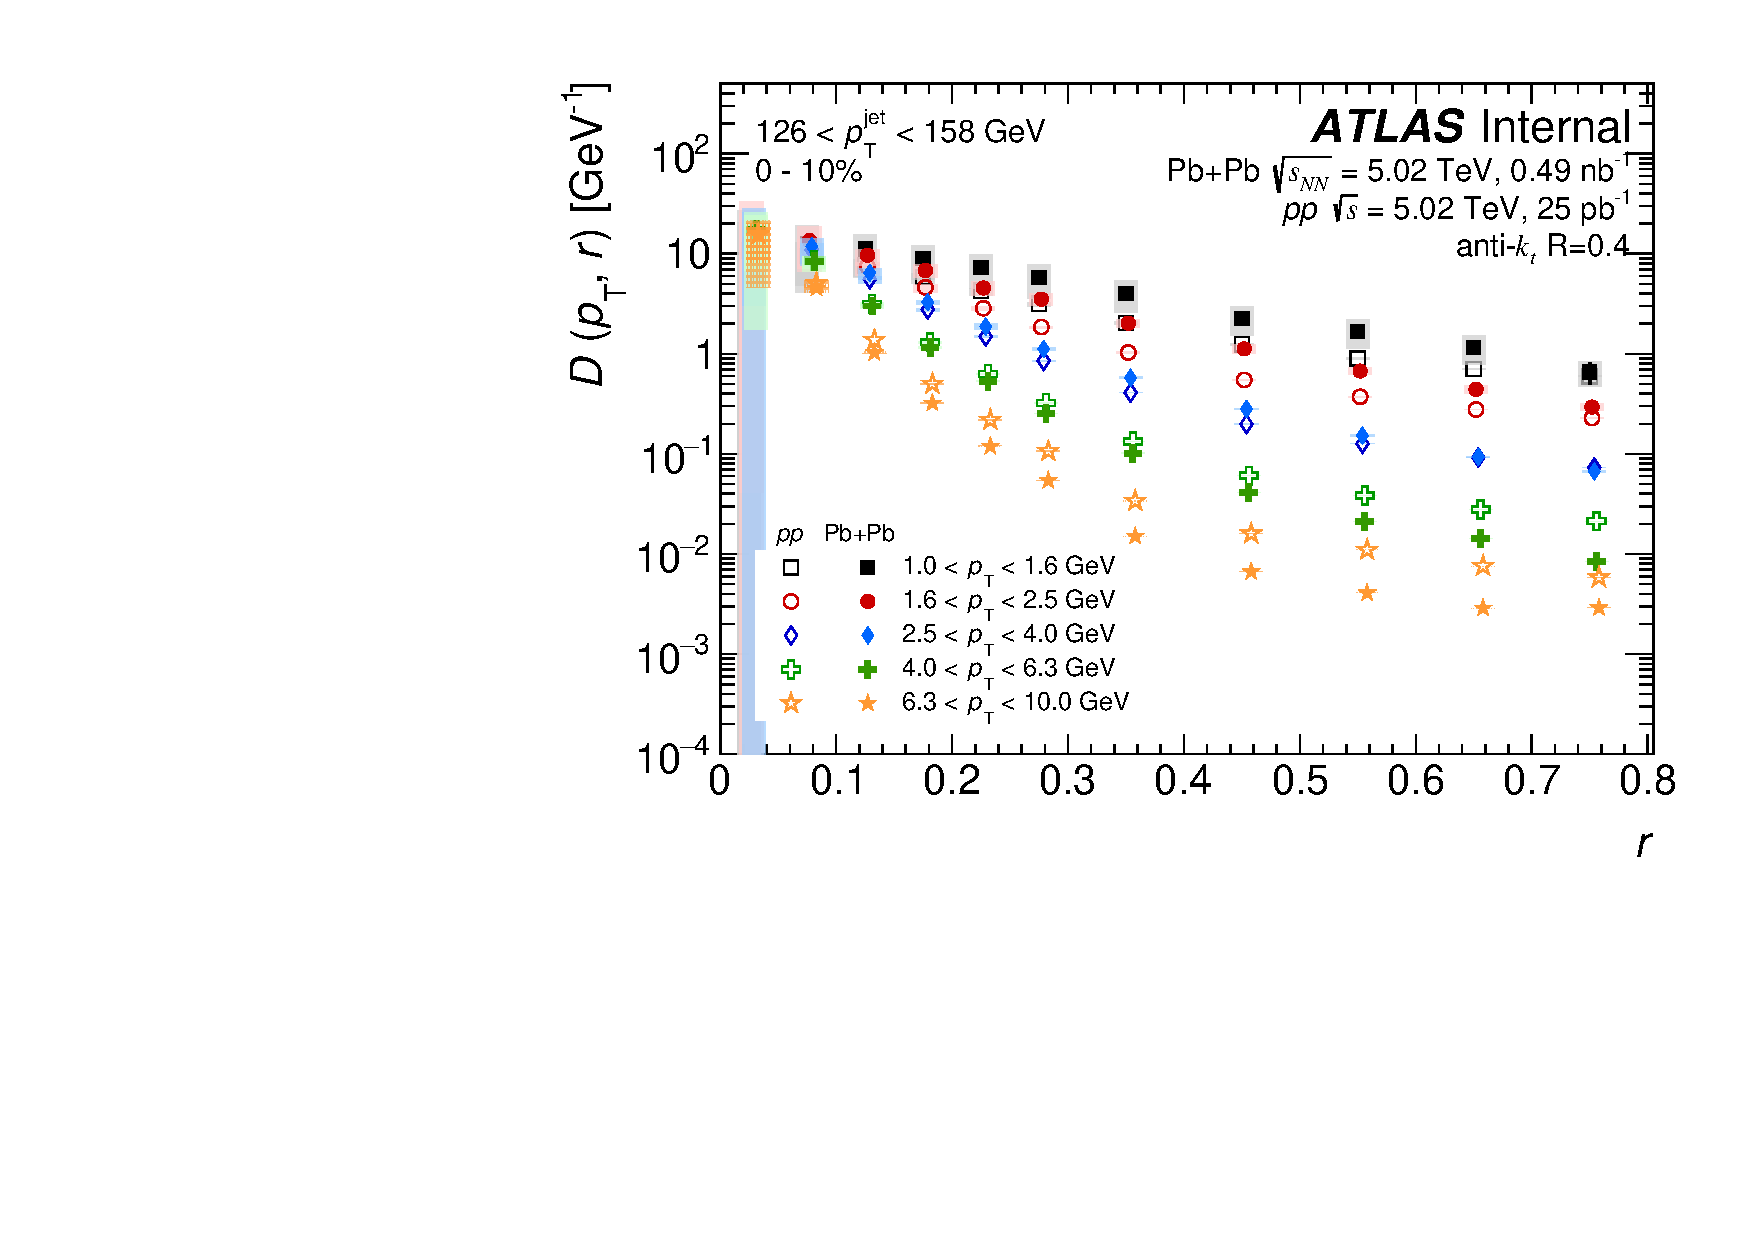
\includegraphics[width=0.45\textwidth]{figures_results/ChPS_final_dR_CONF_DpT_data_jet7_cent0} &
	 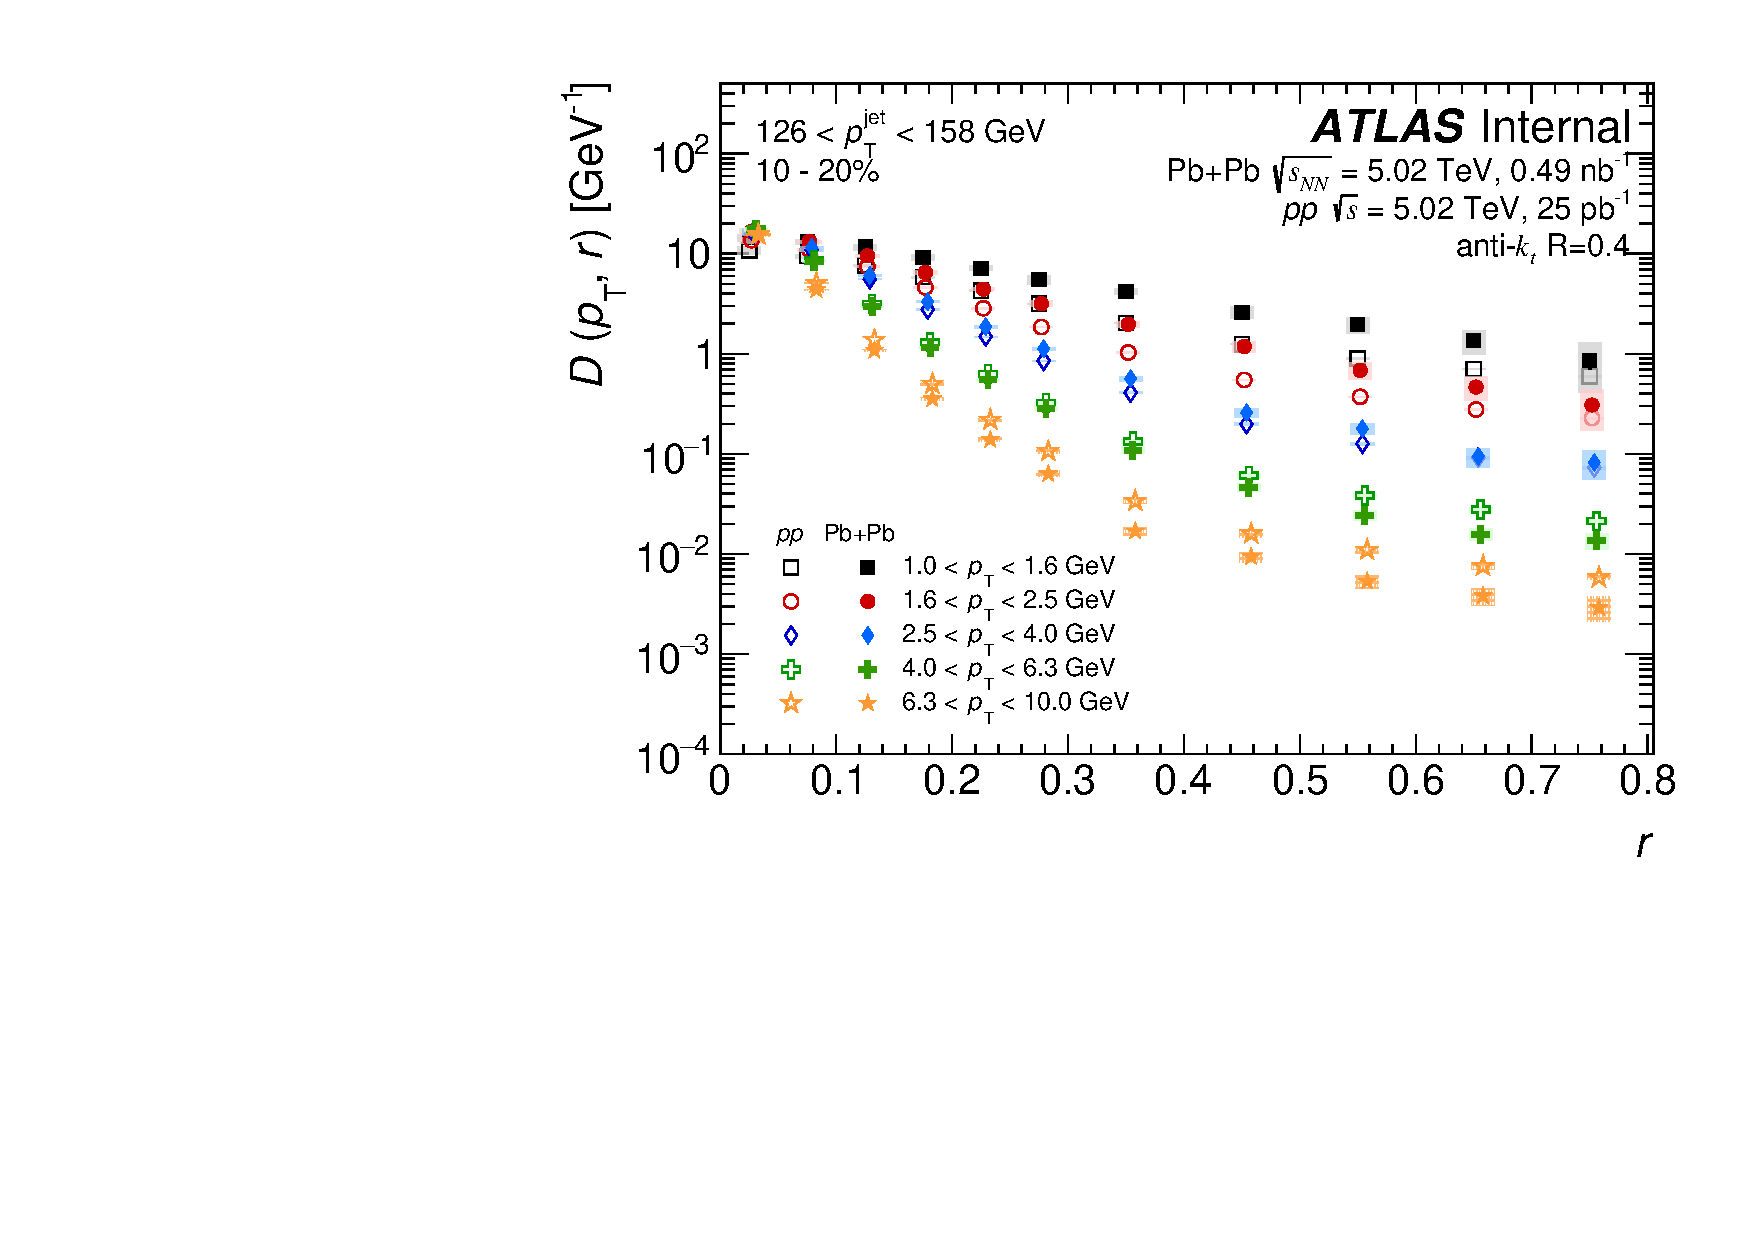
\includegraphics[width=0.45\textwidth]{figures_results/ChPS_final_dR_CONF_DpT_data_jet7_cent1} \\
	 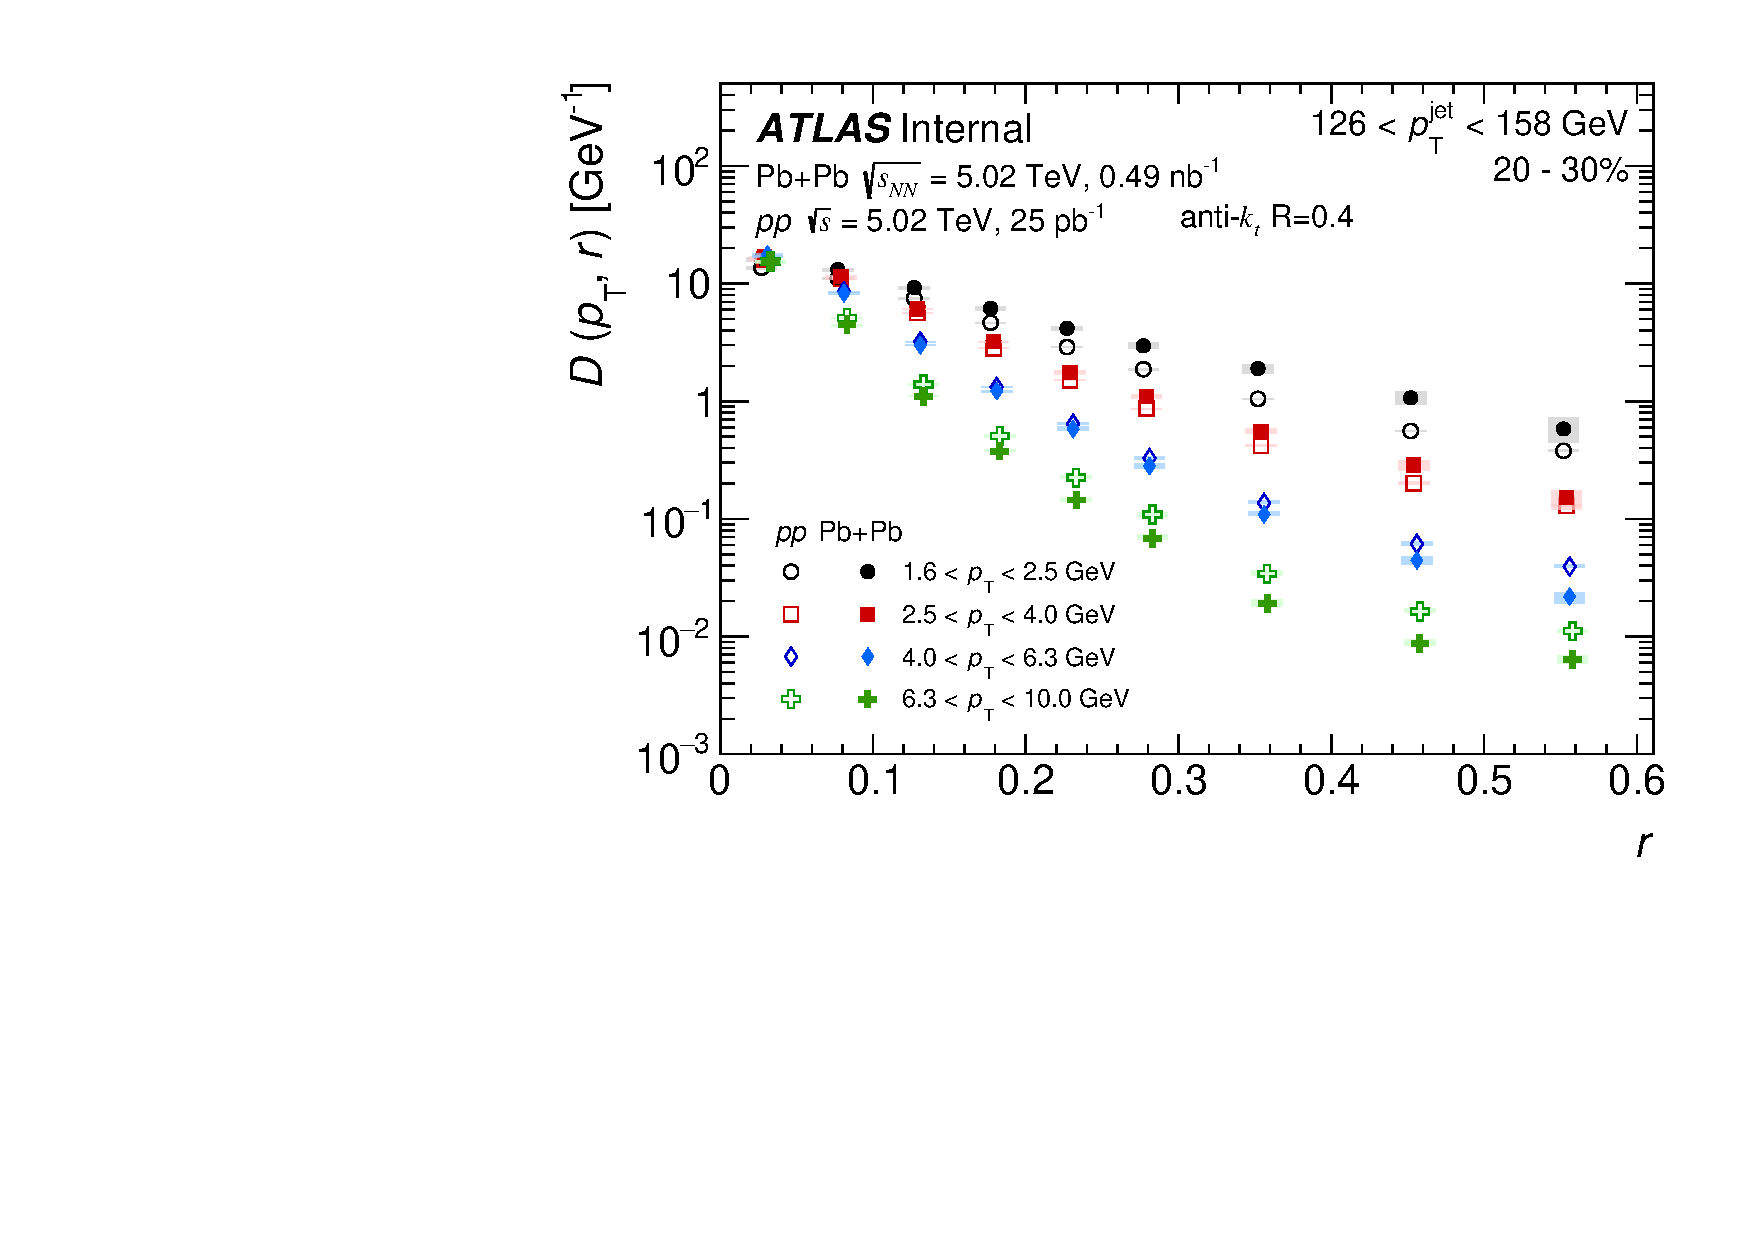
\includegraphics[width=0.45\textwidth]{figures_results/ChPS_final_dR_CONF_DpT_data_jet7_cent2} &
	 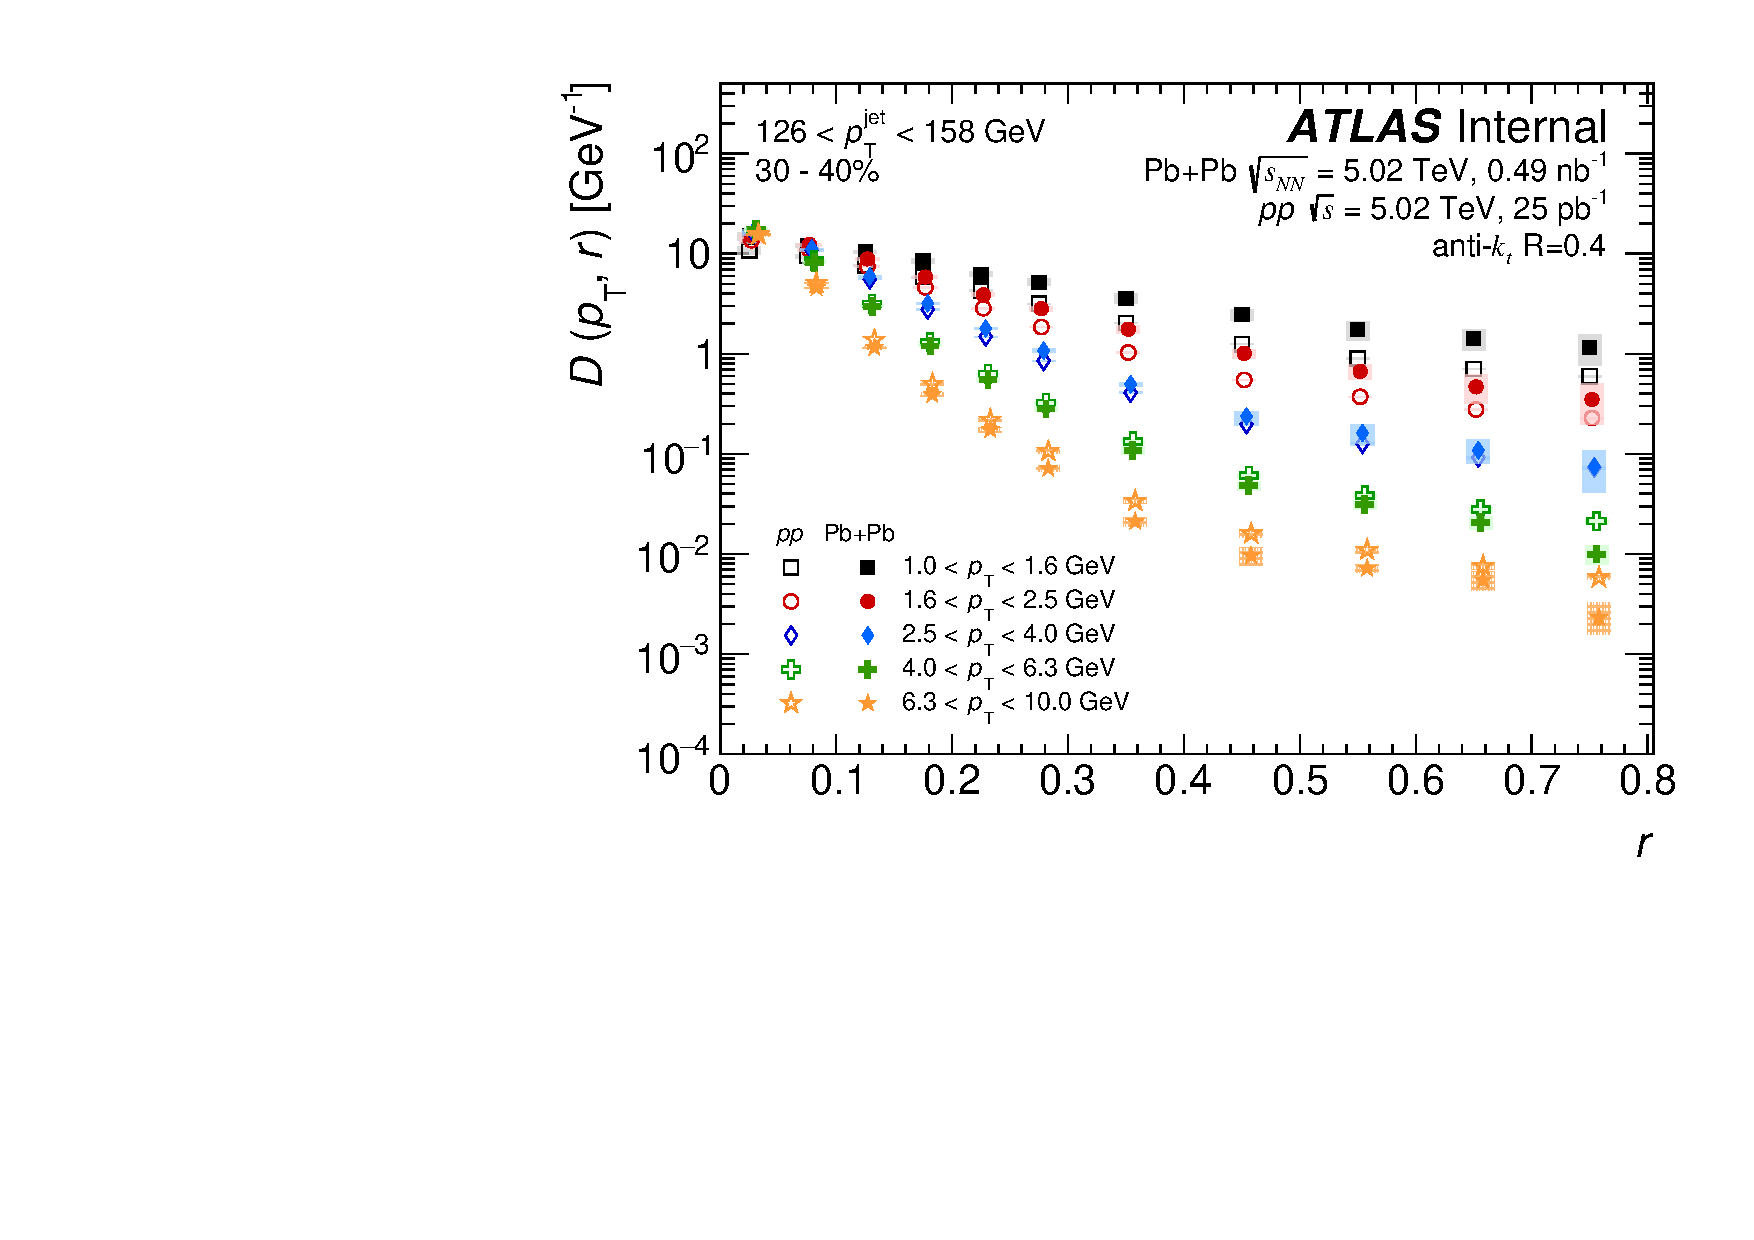
\includegraphics[width=0.45\textwidth]{figures_results/ChPS_final_dR_CONF_DpT_data_jet7_cent3} \\
	 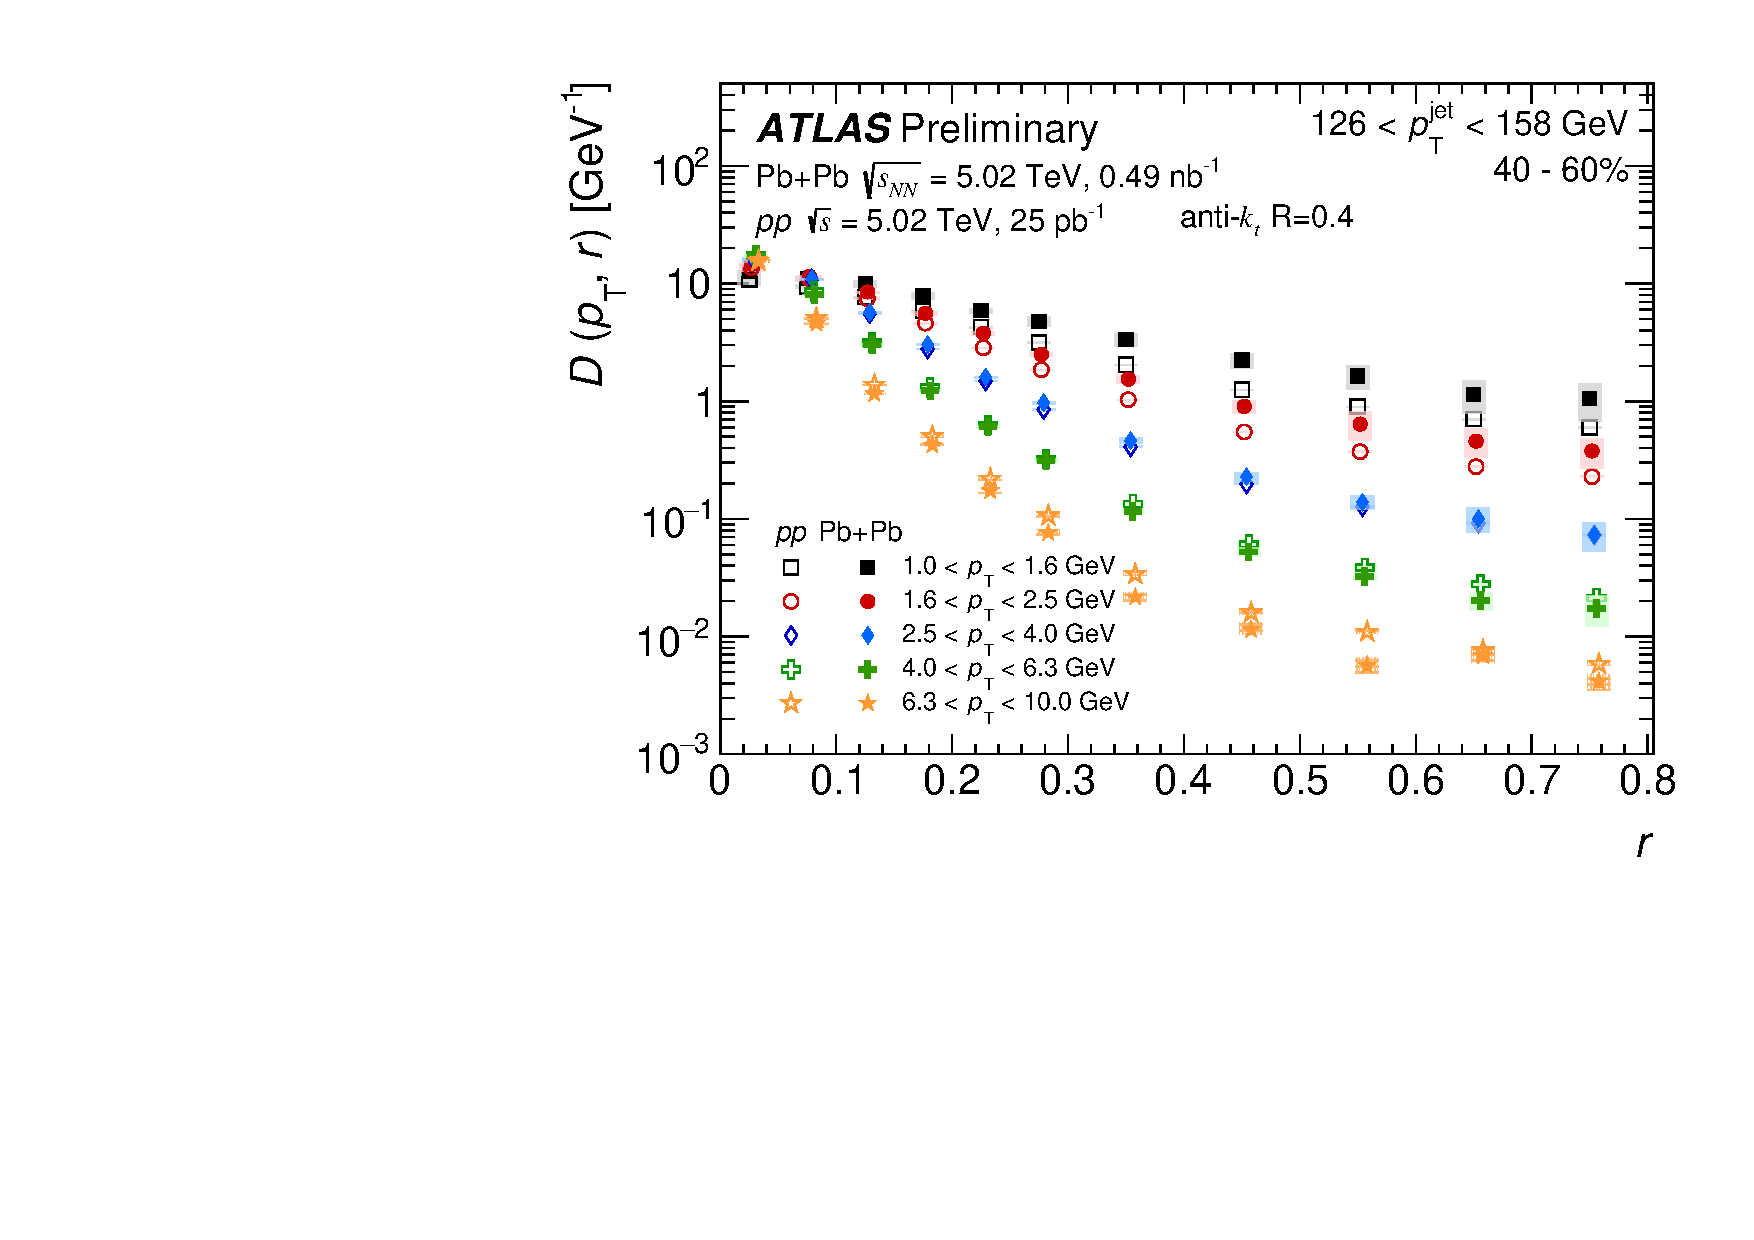
\includegraphics[width=0.45\textwidth]{figures_results/ChPS_final_dR_CONF_DpT_data_jet7_cent4} &
	 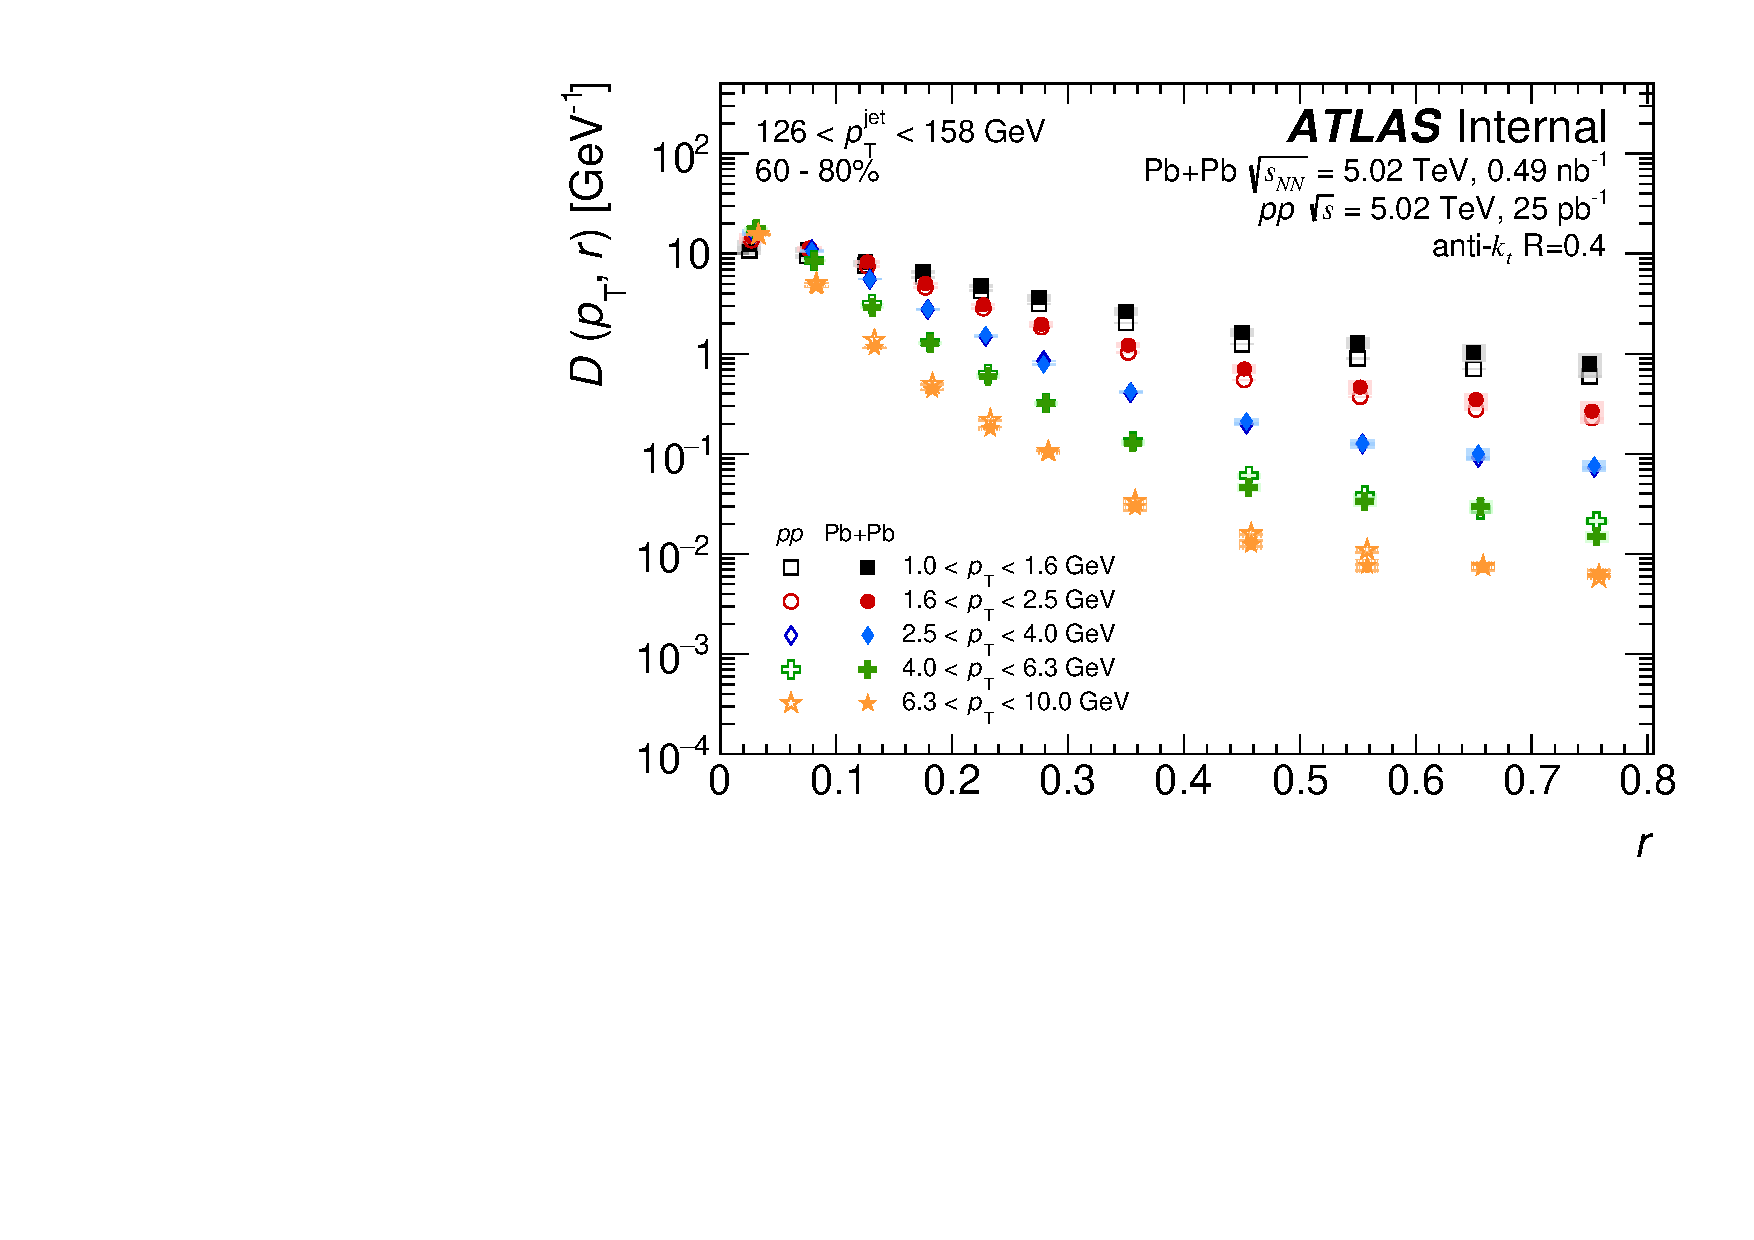
\includegraphics[width=0.45\textwidth]{figures_results/ChPS_final_dR_CONF_DpT_data_jet7_cent5} \\
\end{tabular} }
   \caption{ \Dptr\ as a function of \rvar\ for different centrality bins for charged particles with five different track \pT\ ranges (1.0--1.6~\GeV\, 1.6--2.5~\GeV\, 2.5--4.0~\GeV\, 4.0--6.3~\GeV\, 6.3--10.0~\GeV\ ), for jets with \pt\ 126--158 \GeV\, along with the corresponding \Dptr\ distributions from \pp\ collisions overlaid. }
      \label{fig:dptr_pbpb_pp}
\end{figure}



Figure~\ref{fig:rdptcent} shows \RDptr\ as a function of \rvar\ for seven \pt\ selections: 1.0--1.6~\GeV, 1.6--2.5~\GeV, 2.5--4.0~\GeV, 4.0--6.3~\GeV, 6.3--10.0~\GeV, 10.0--25.1~\GeV\ and 25.1--63.1~\GeV\ for \pbpb\ collisions in all centrality bins. It can be seen that in central collisions, charged particles
with $\pt <$~4.0~\GeV, \RDptr\ grows with increasing \rvar\ for $r <0.3$, is approximately constant for
$0.3 < r <0.6$, and goes down for $0.6 < r < 0.8$.  For $\pt > $~4.0~\GeV\ \RDptr\ decreases with increasing \rvar\ for $ r < 0.3$
and is approximately constant for $ 0.3 < r <0.8$.
For peripheral collisions, \RDptr\ has an enhancement for the lowest \pt\ particles ($\pt < 2.5$ GeV), with higher \pt\ particles showing a decreasing \RDptr\ with increasing \rvar. Intermediate \pt\ particles ($2.5 < \pt < 10 $ GeV) do not show any significant \rvar\ dependence.

\begin{figure}
\centering{
\begin{tabular}{cc}
	 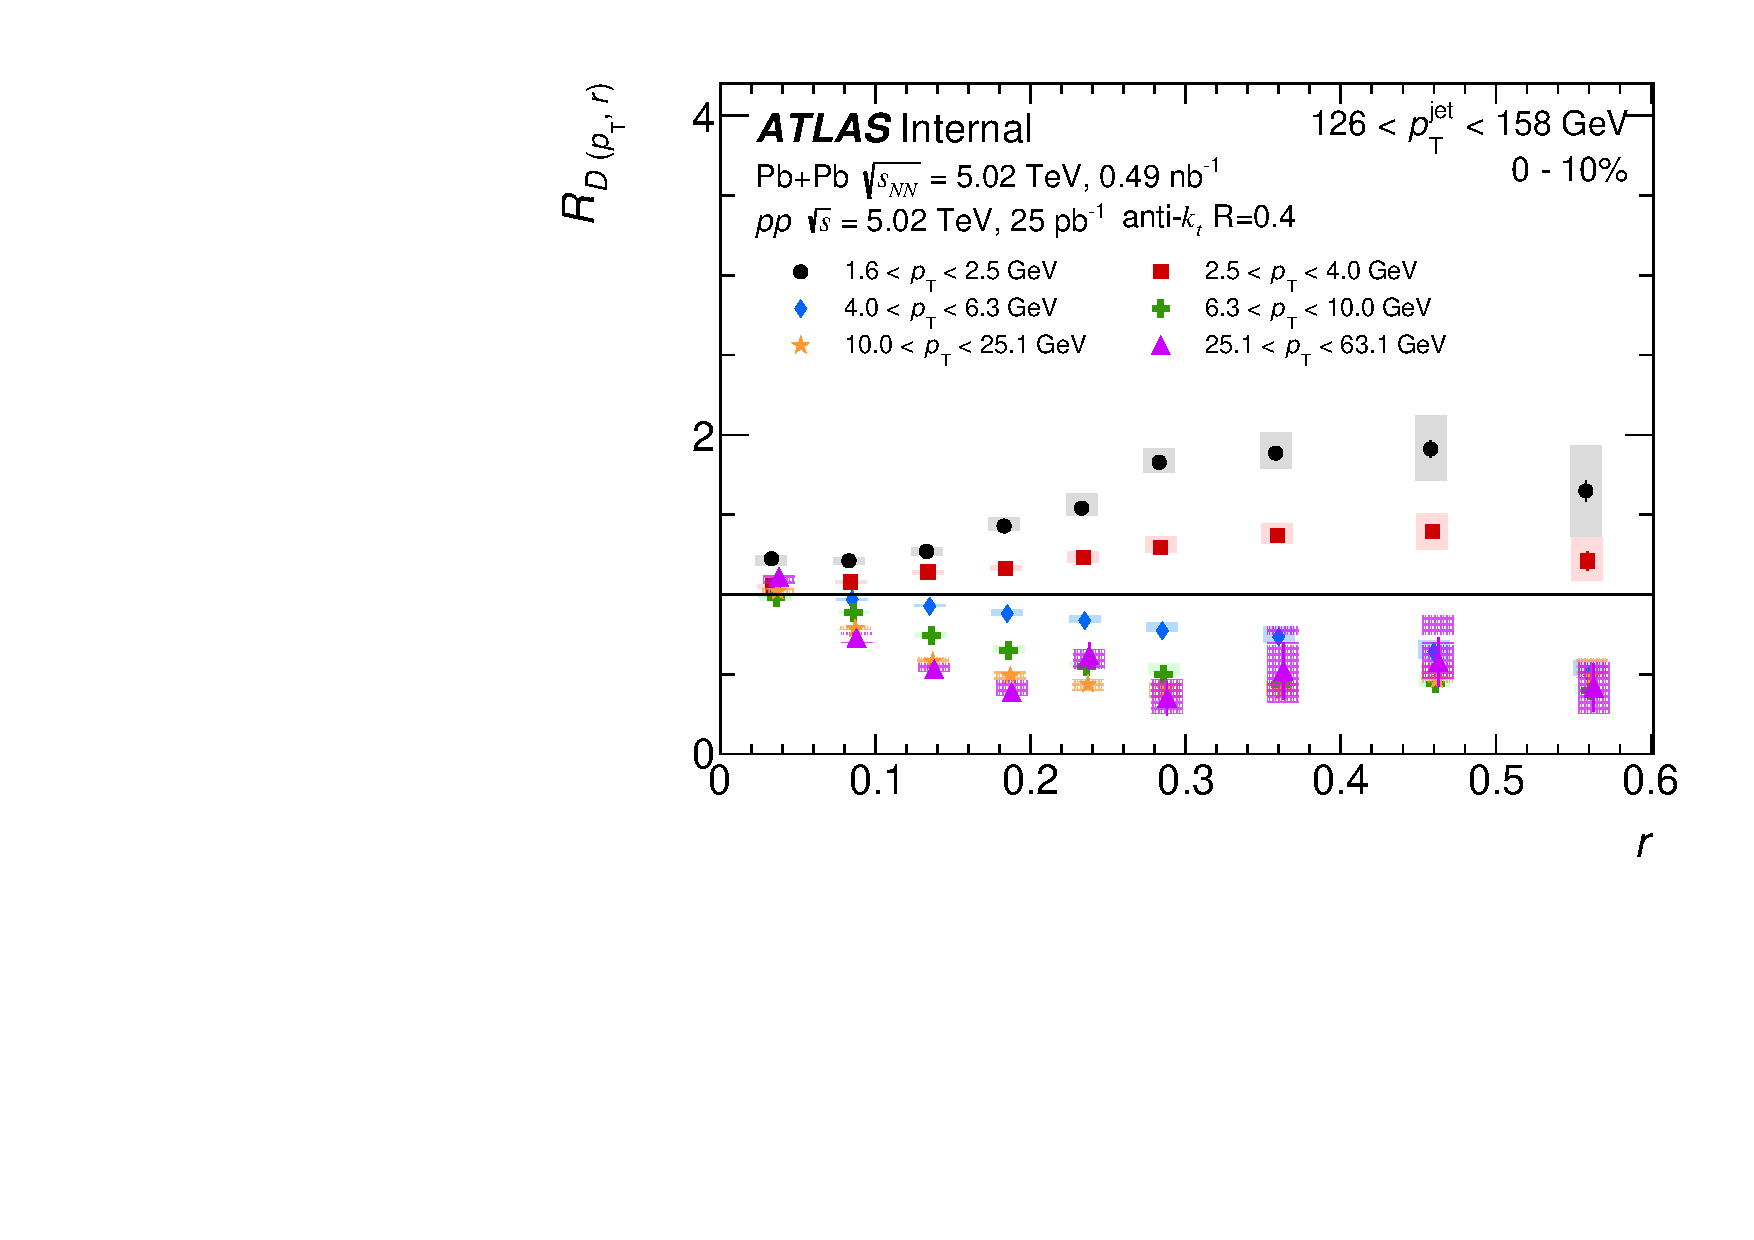
\includegraphics[width=0.45\textwidth]{figures_results/RDpT_final_ratio_dR_CONF_data_jet7_cent0} &
	 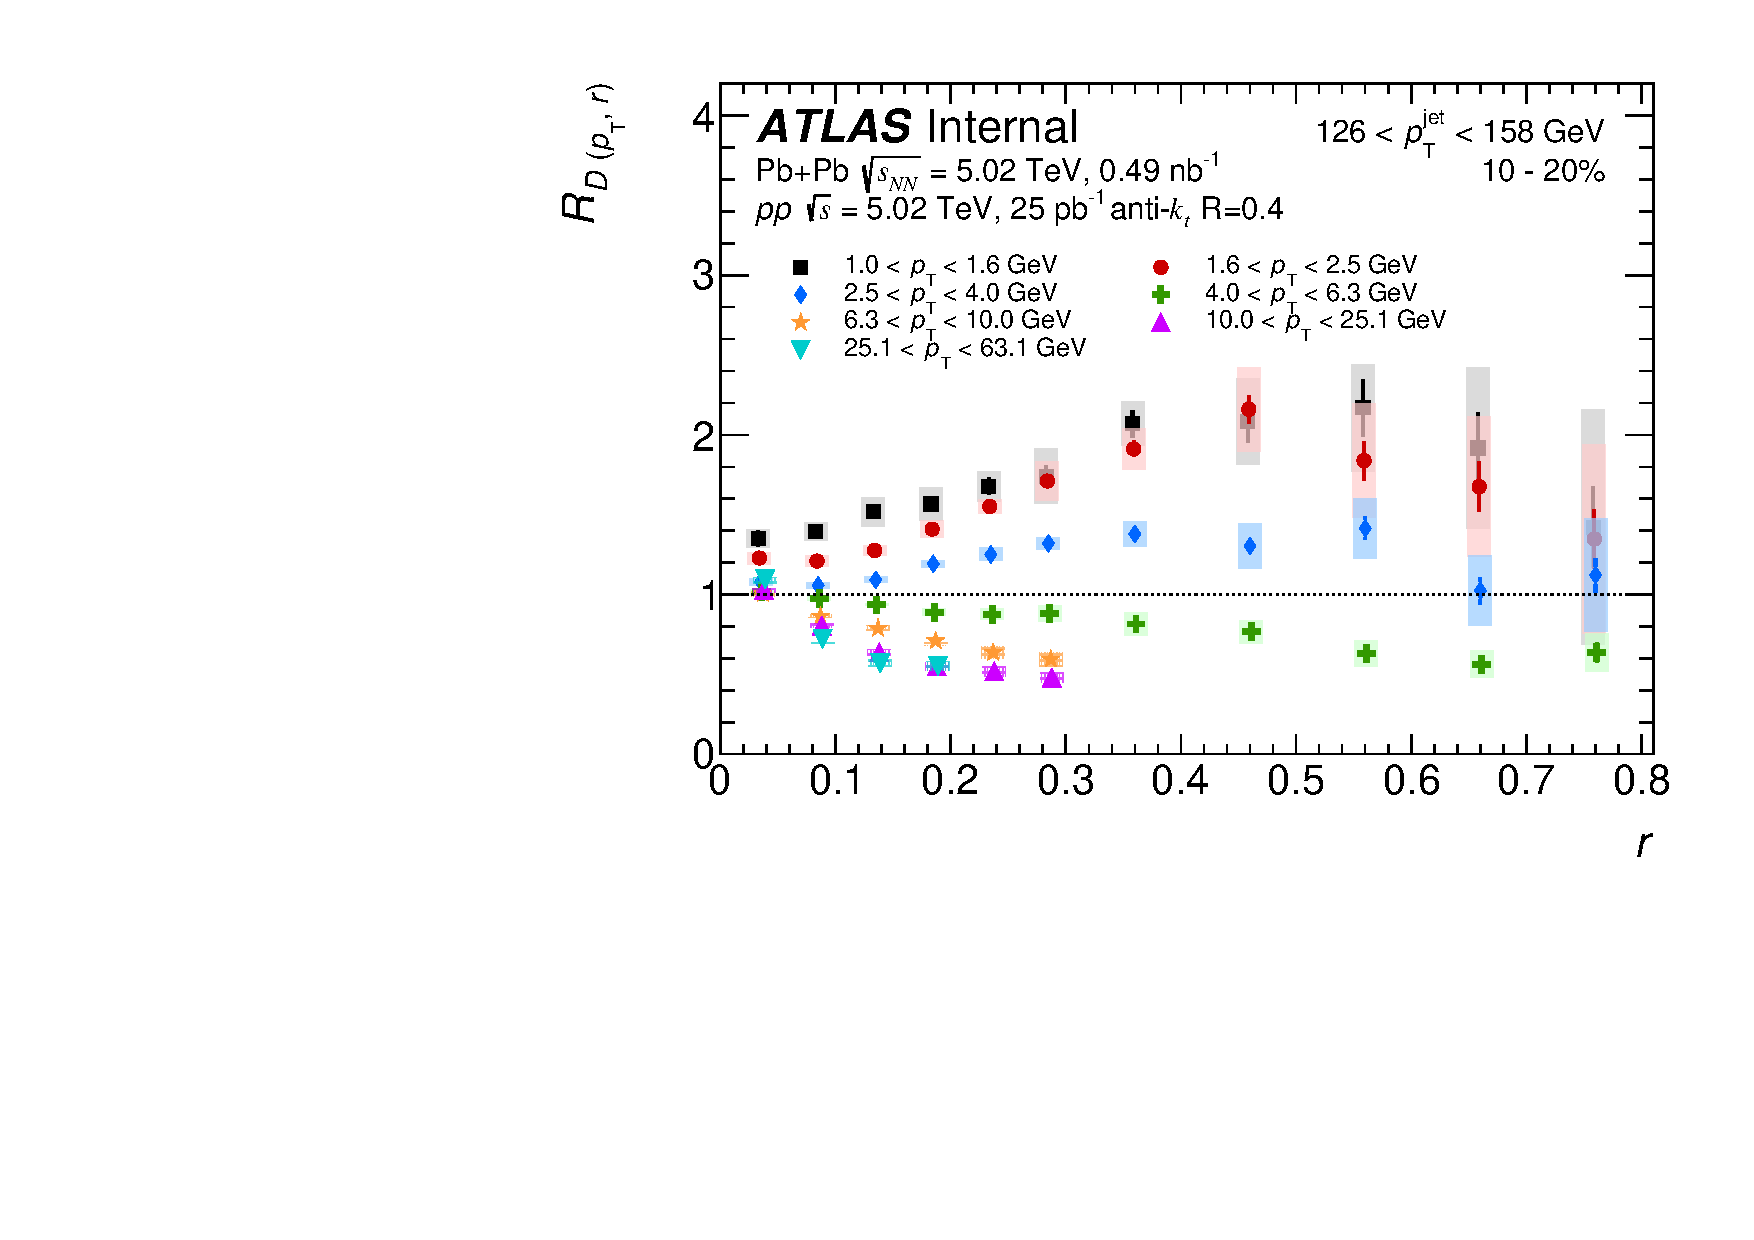
\includegraphics[width=0.45\textwidth]{figures_results/RDpT_final_ratio_dR_CONF_data_jet7_cent1} \\
	 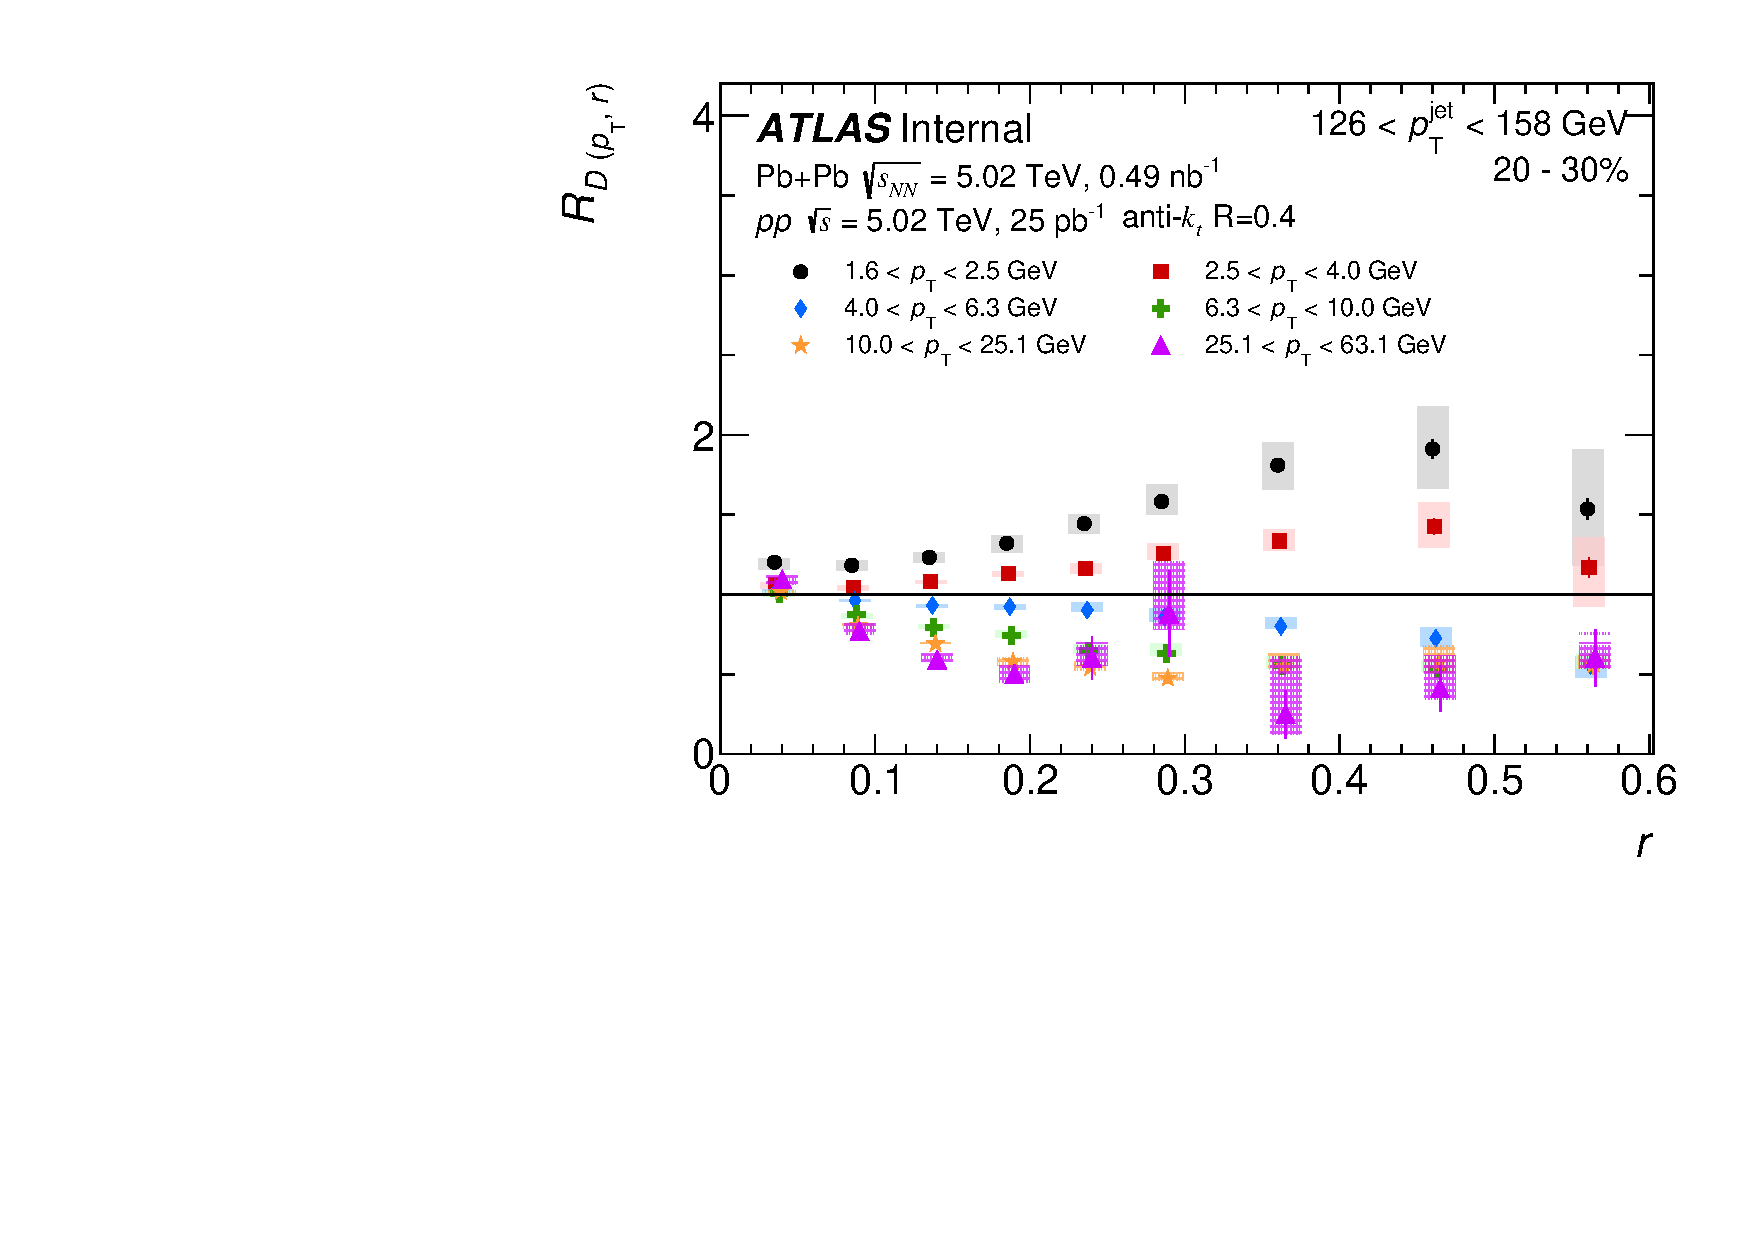
\includegraphics[width=0.45\textwidth]{figures_results/RDpT_final_ratio_dR_CONF_data_jet7_cent2} &
	 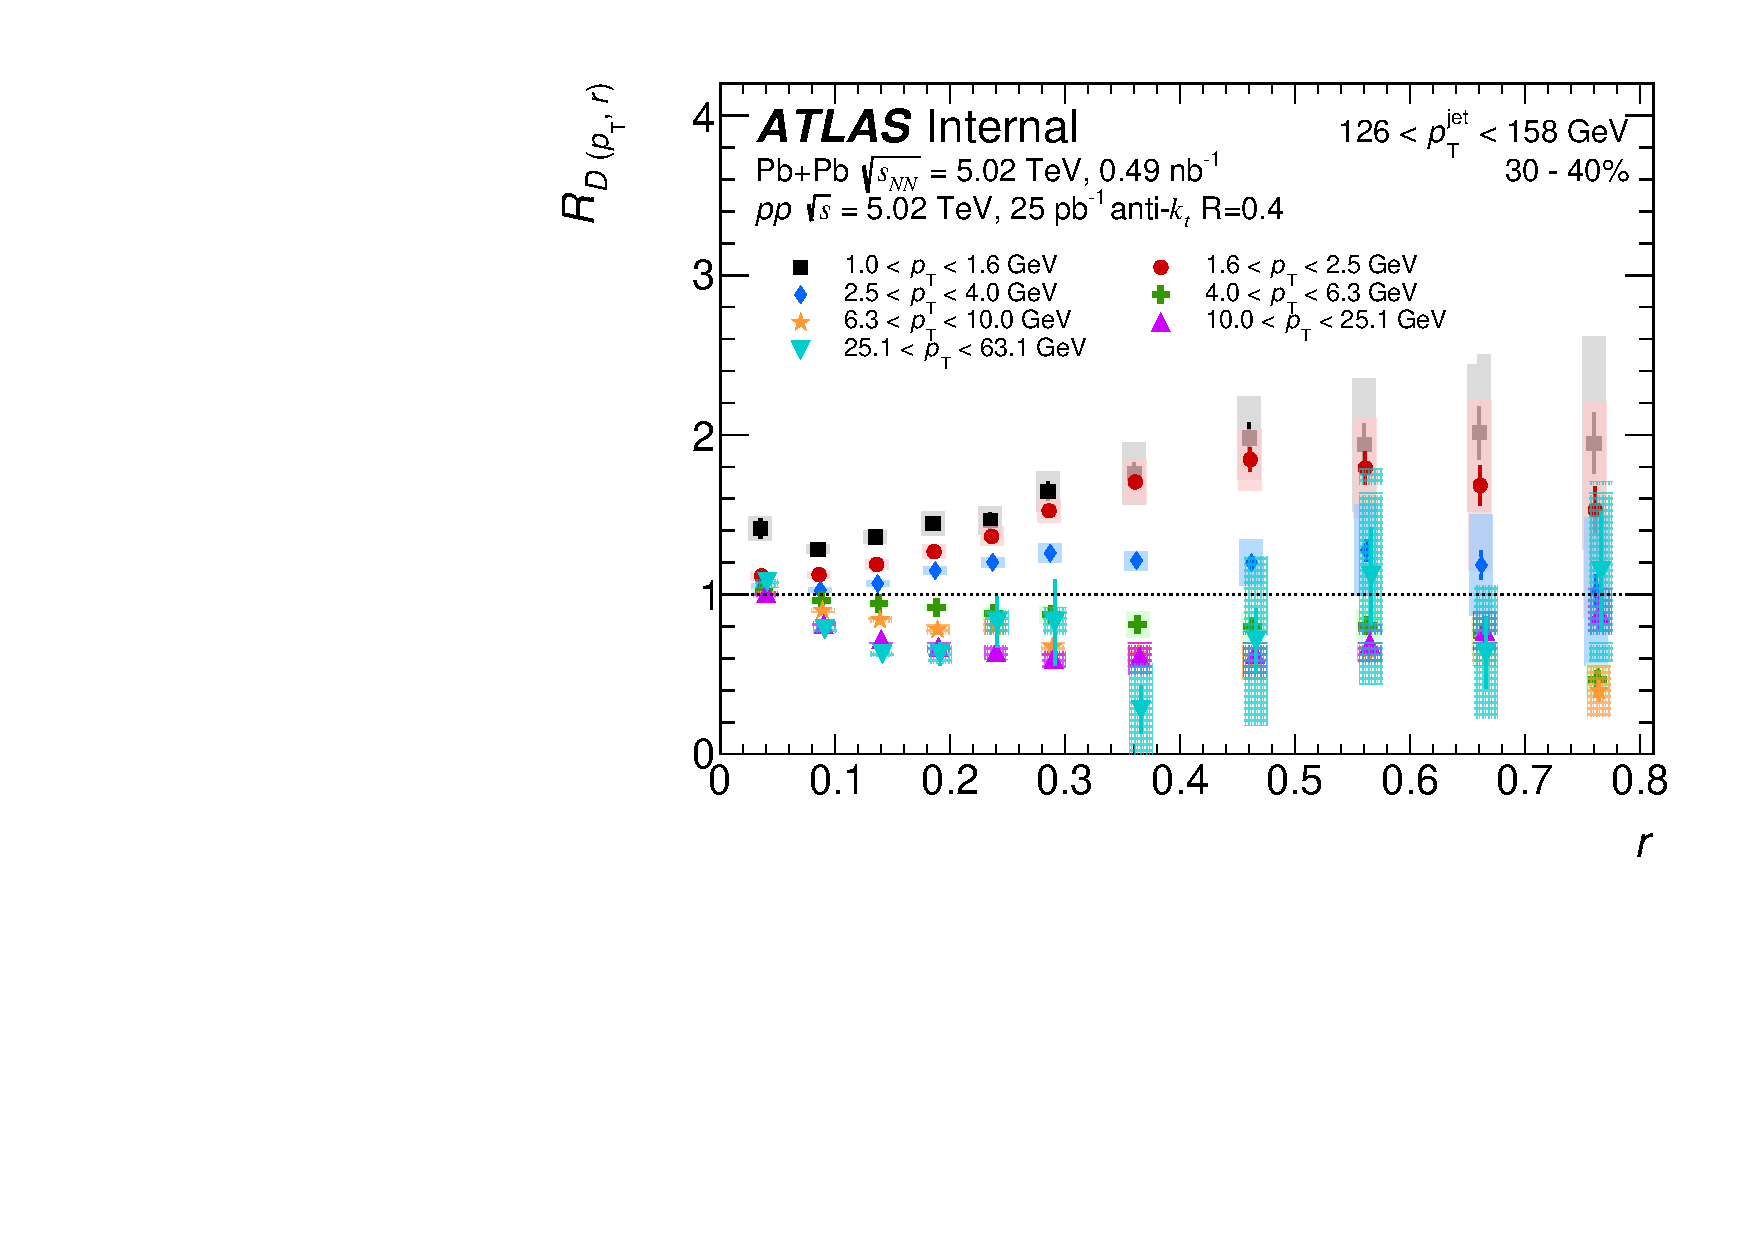
\includegraphics[width=0.45\textwidth]{figures_results/RDpT_final_ratio_dR_CONF_data_jet7_cent3} \\
	 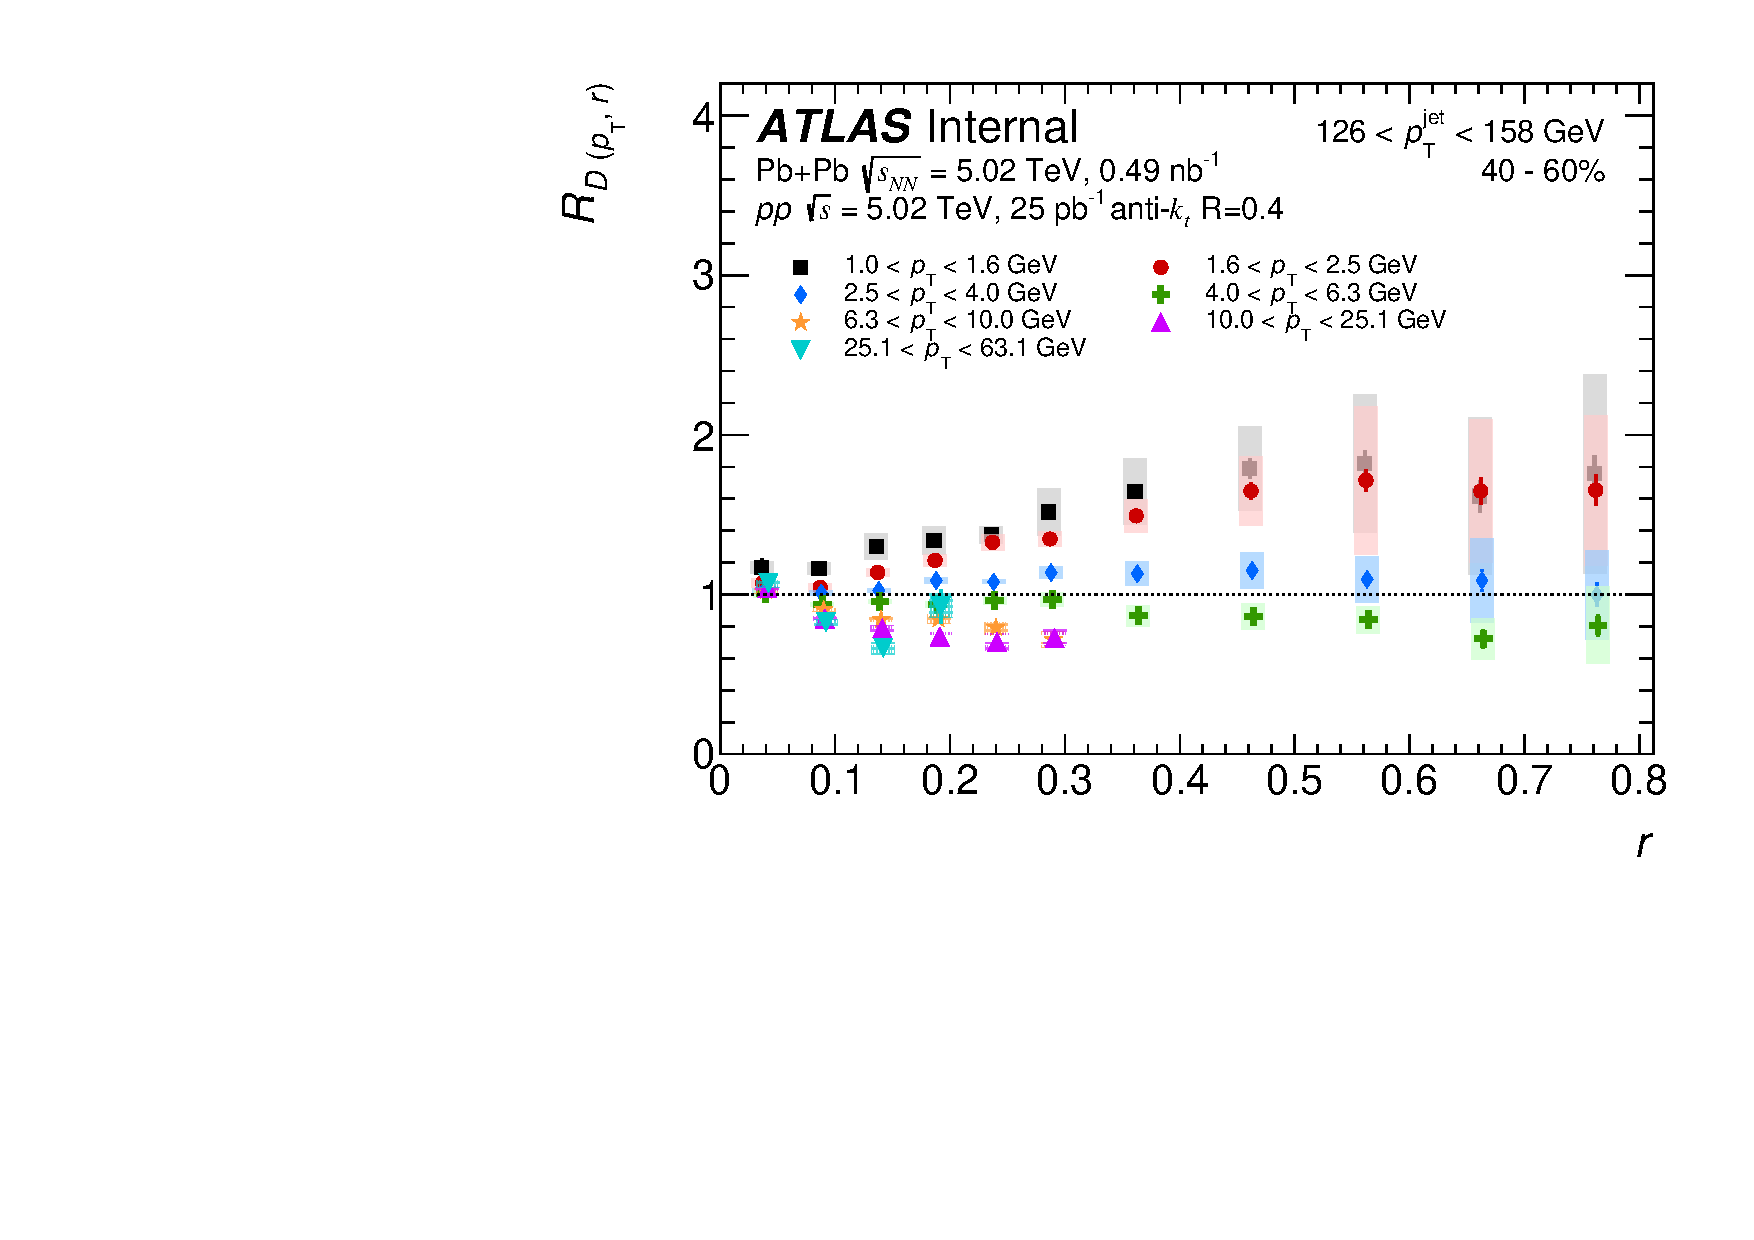
\includegraphics[width=0.45\textwidth]{figures_results/RDpT_final_ratio_dR_CONF_data_jet7_cent4} &
	 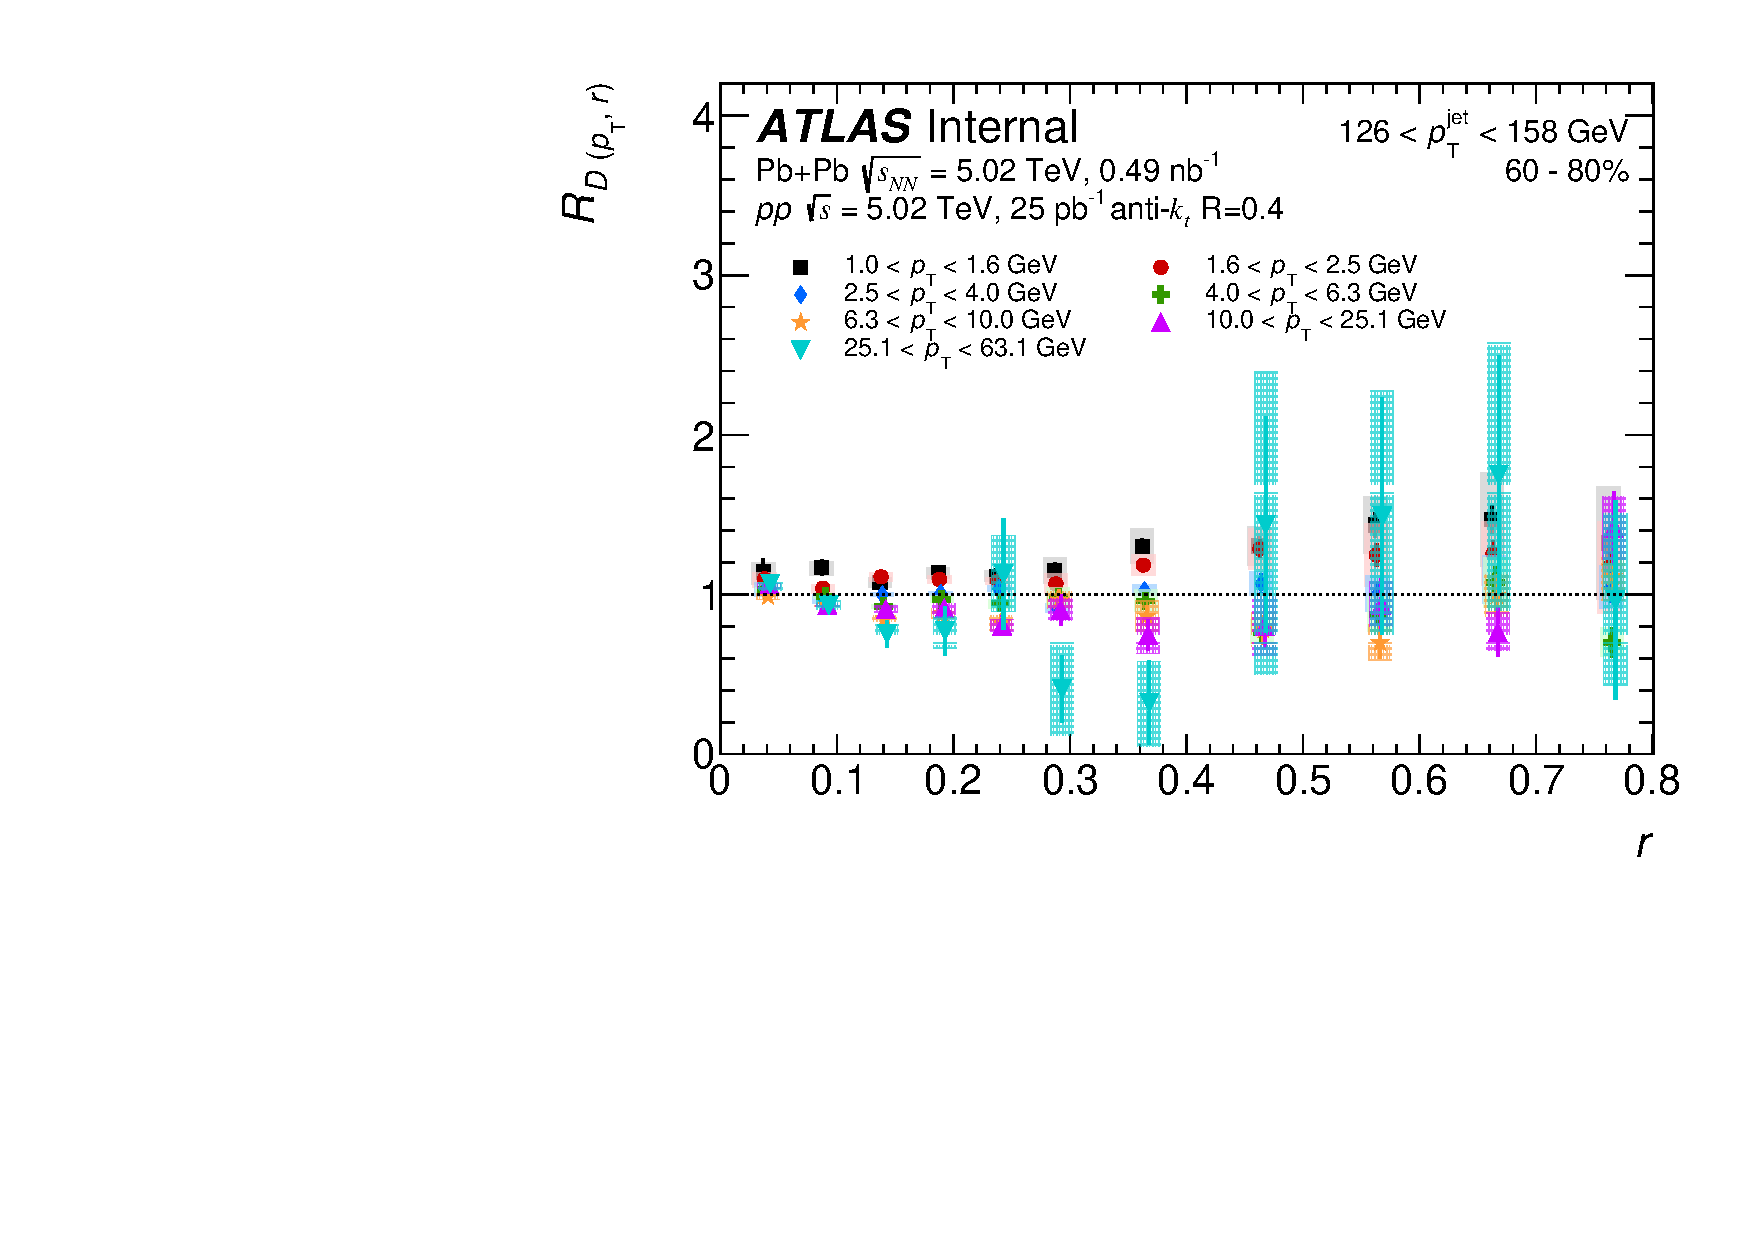
\includegraphics[width=0.45\textwidth]{figures_results/RDpT_final_ratio_dR_CONF_data_jet7_cent5} \\
\end{tabular} }
   \caption{\RDptr\ for different track \pt\ ranges, as a function of \rvar\ for different centrality ranges.}
      \label{fig:rdptcent}
\end{figure}


The \Rdptr\ distribution can be integrated over $ r < 0.4 $, which can then be directly compared to the ATLAS 5 TeV \pbpb\ fragmentation function result \cite{ATLAS502FFConf}. This comparison is shown in Figure~\ref{fig:FF_comparison_jet1}-\ref{fig:FF_comparison_jet4}. It can be seen that both measurements agree within the systematic uncertainties for all \ptjet\ bins used in the analyses. Any differences come from the the different methods of UE estimation used in the two analyses, where even small differences in the UE lead to large variations in the subtracted distributions because of the poor signal to background ratio.

\begin{figure}
\centering{
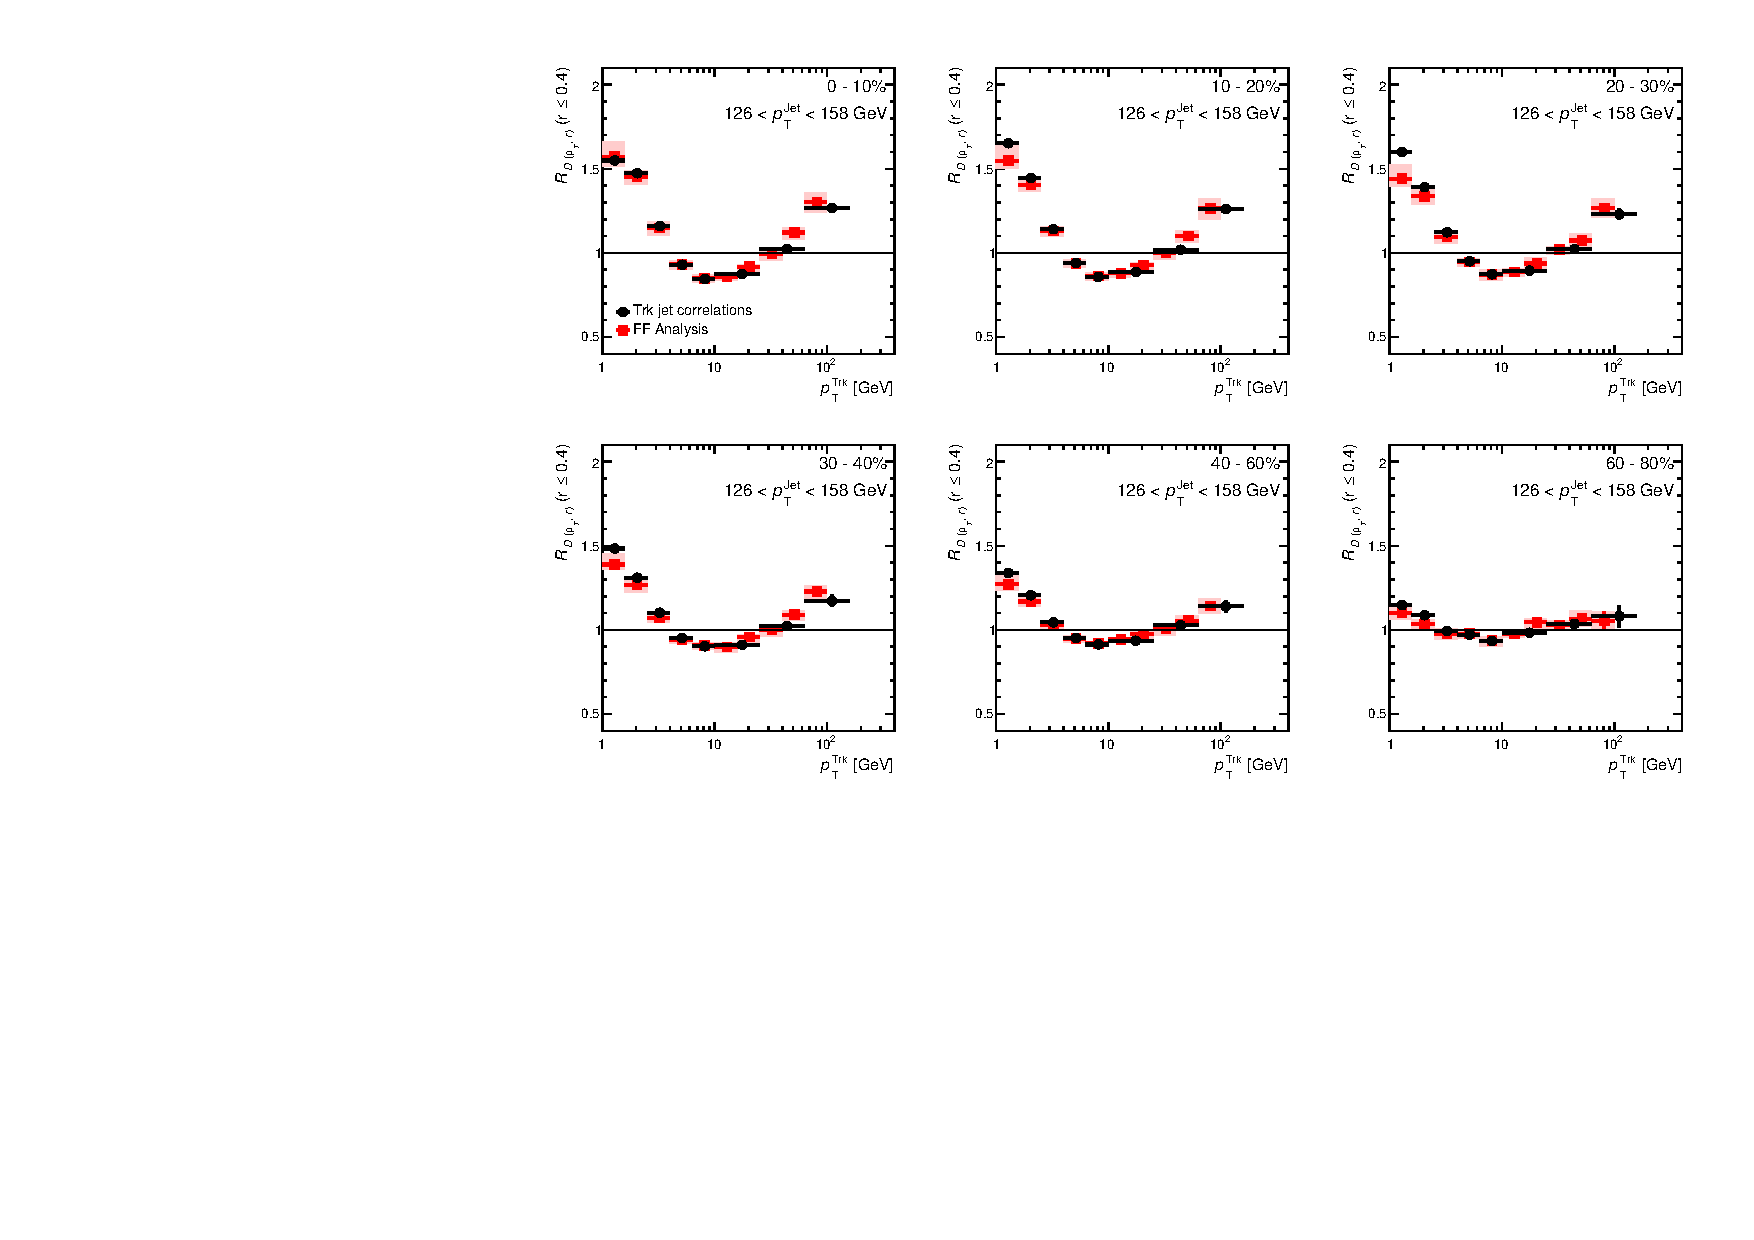
\includegraphics[page=1, width=0.8\textwidth]{figures_results/ChPS_FF_final_injet_ratio_data} \\
 }
\caption{\Rdptr\ integrated over $ r < 0.4$ and overlaid on top of the fragmentation function distributions as measured in \cite{ATLAS502FFConf}. The comparison is shown as a function of track \pt, for \ptjet\ 126--158 \GeV\,  for different centrality bins }
\label{fig:FF_comparison_jet1}
\end{figure}

\begin{figure}
\centering{
\includegraphics[page=2, width=0.8\textwidth]{figures_results/ChPS_FF_final_injet_ratio_data} \\
 }
\caption{\Rdptr\ integrated over $ r < 0.4$ and overlaid on top of the fragmentation function distributions as measured in \cite{ATLAS502FFConf}. The comparison is shown as a function of track \pt, for  \ptjet\ 158--200 \GeV\,  for different centrality bins }
\label{fig:FF_comparison_jet2}
\end{figure}

\begin{figure}
\centering{
\includegraphics[page=3, width=0.8\textwidth]{figures_results/ChPS_FF_final_injet_ratio_data} \\
 }
\caption{\Rdptr\ integrated over $ r < 0.4$ and overlaid on top of the fragmentation function distributions as measured in \cite{ATLAS502FFConf}. The comparison is shown as a function of track \pt, for \ptjet\ 200--251 \GeV\,  for different centrality bins }
\label{fig:FF_comparison_jet3}
\end{figure}

\begin{figure}
\centering{
\includegraphics[page=4, width=0.8\textwidth]{figures_results/ChPS_FF_final_injet_ratio_data} \\
 }
\caption{\Rdptr\ integrated over $ r < 0.4$ and overlaid on top of the fragmentation function distributions as measured in \cite{ATLAS502FFConf}. The comparison is shown as a function of track \pt, for \ptjet\ 251--315 \GeV\,  for different centrality bins }
\label{fig:FF_comparison_jet4}
\end{figure}


Figure~\ref{fig:ptjetdep} shows the \ptjet\ dependence of \RDptr\ for two \pt\ selections: 1.0--1.6~\GeV\ and
6.3--10.0~\GeV.  Charged particles from the lower \pt\ selection have an \RDptr\ which increases as 
with increasing \ptjet\ at all  \rvar.  The higher \pt\ charged particles
have an \RDptr\ value which decreases with increasing \rvar, but which is consistent for all \ptjet\ selections.



\begin{figure}
\centering{
\begin{tabular}{cc}
	 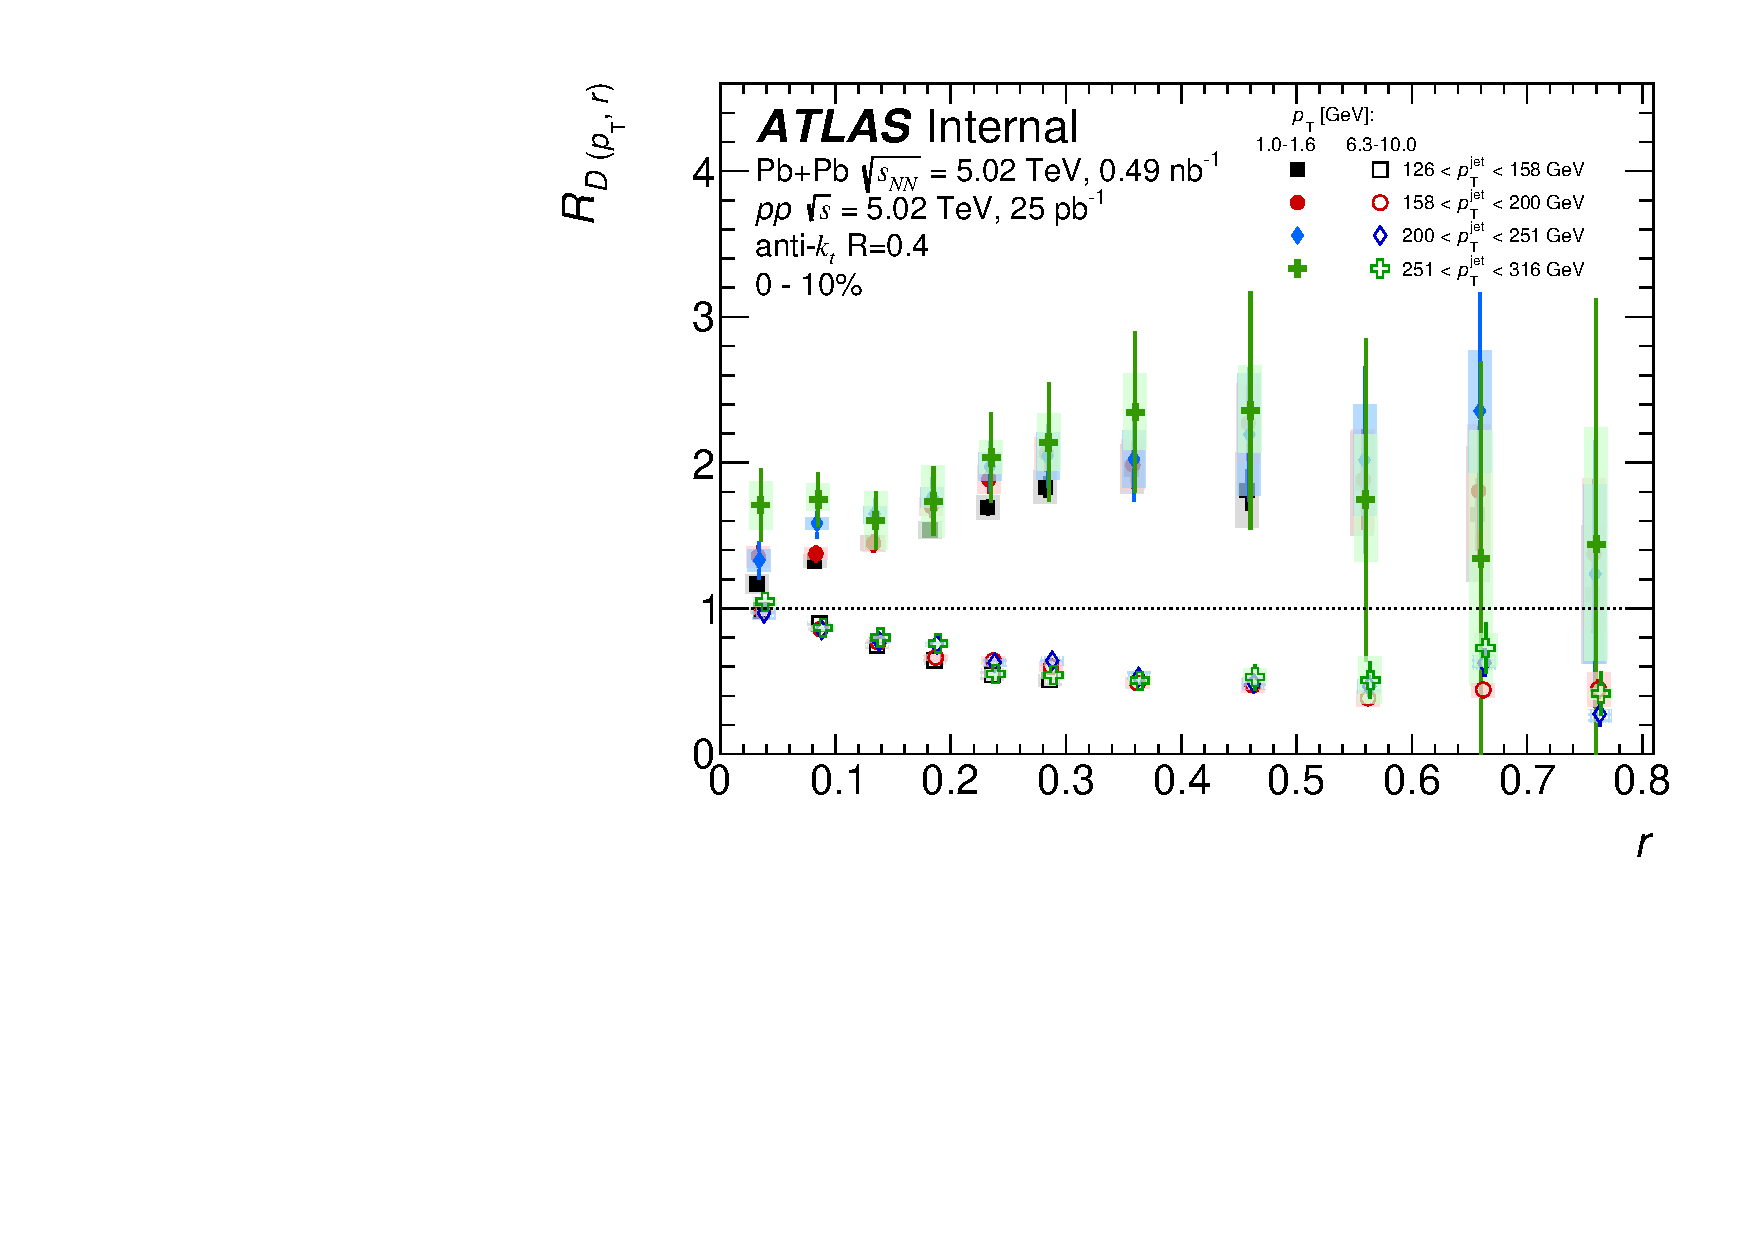
\includegraphics[width=0.45\textwidth]{figures_results/RDpT_final_ratio_dR_CONF_data_trk2_6_cent0} &
	 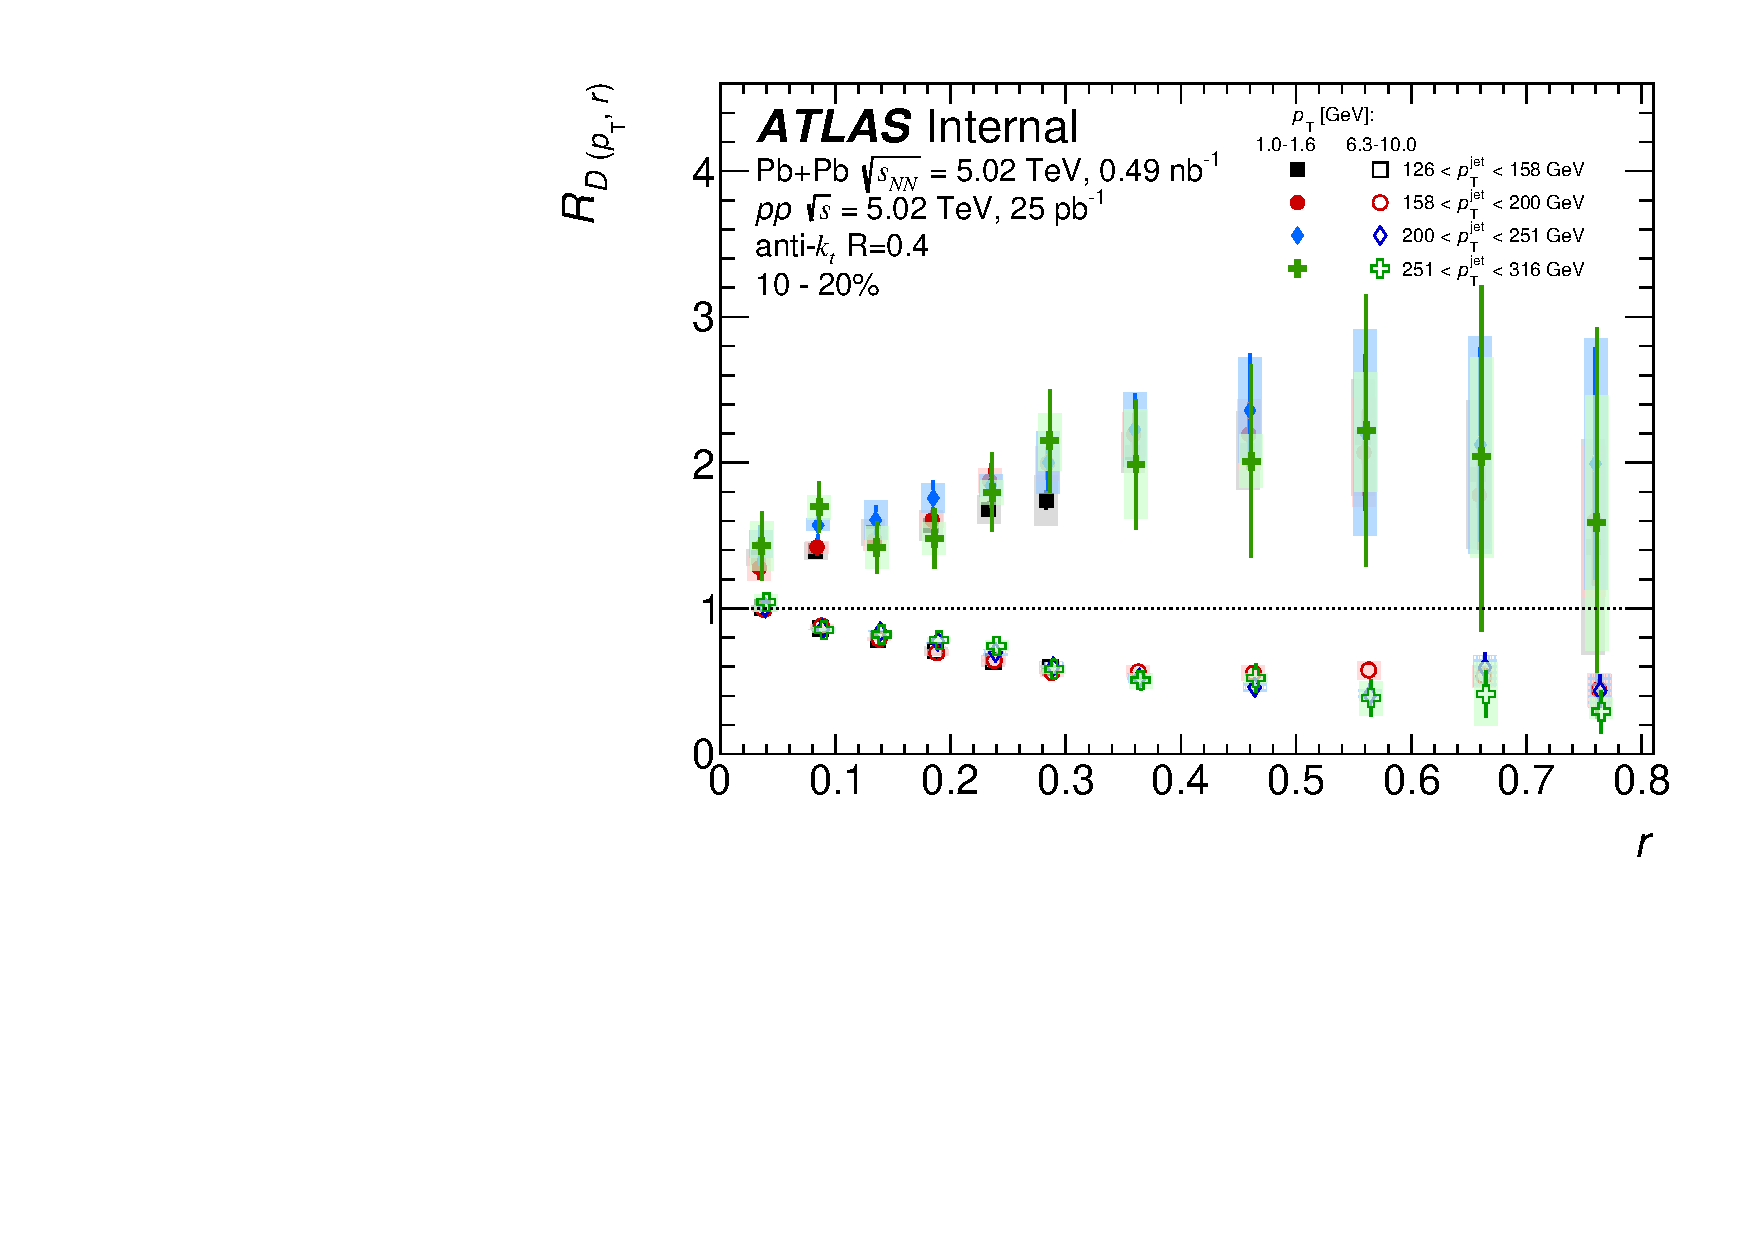
\includegraphics[width=0.45\textwidth]{figures_results/RDpT_final_ratio_dR_CONF_data_trk2_6_cent1} \\
	 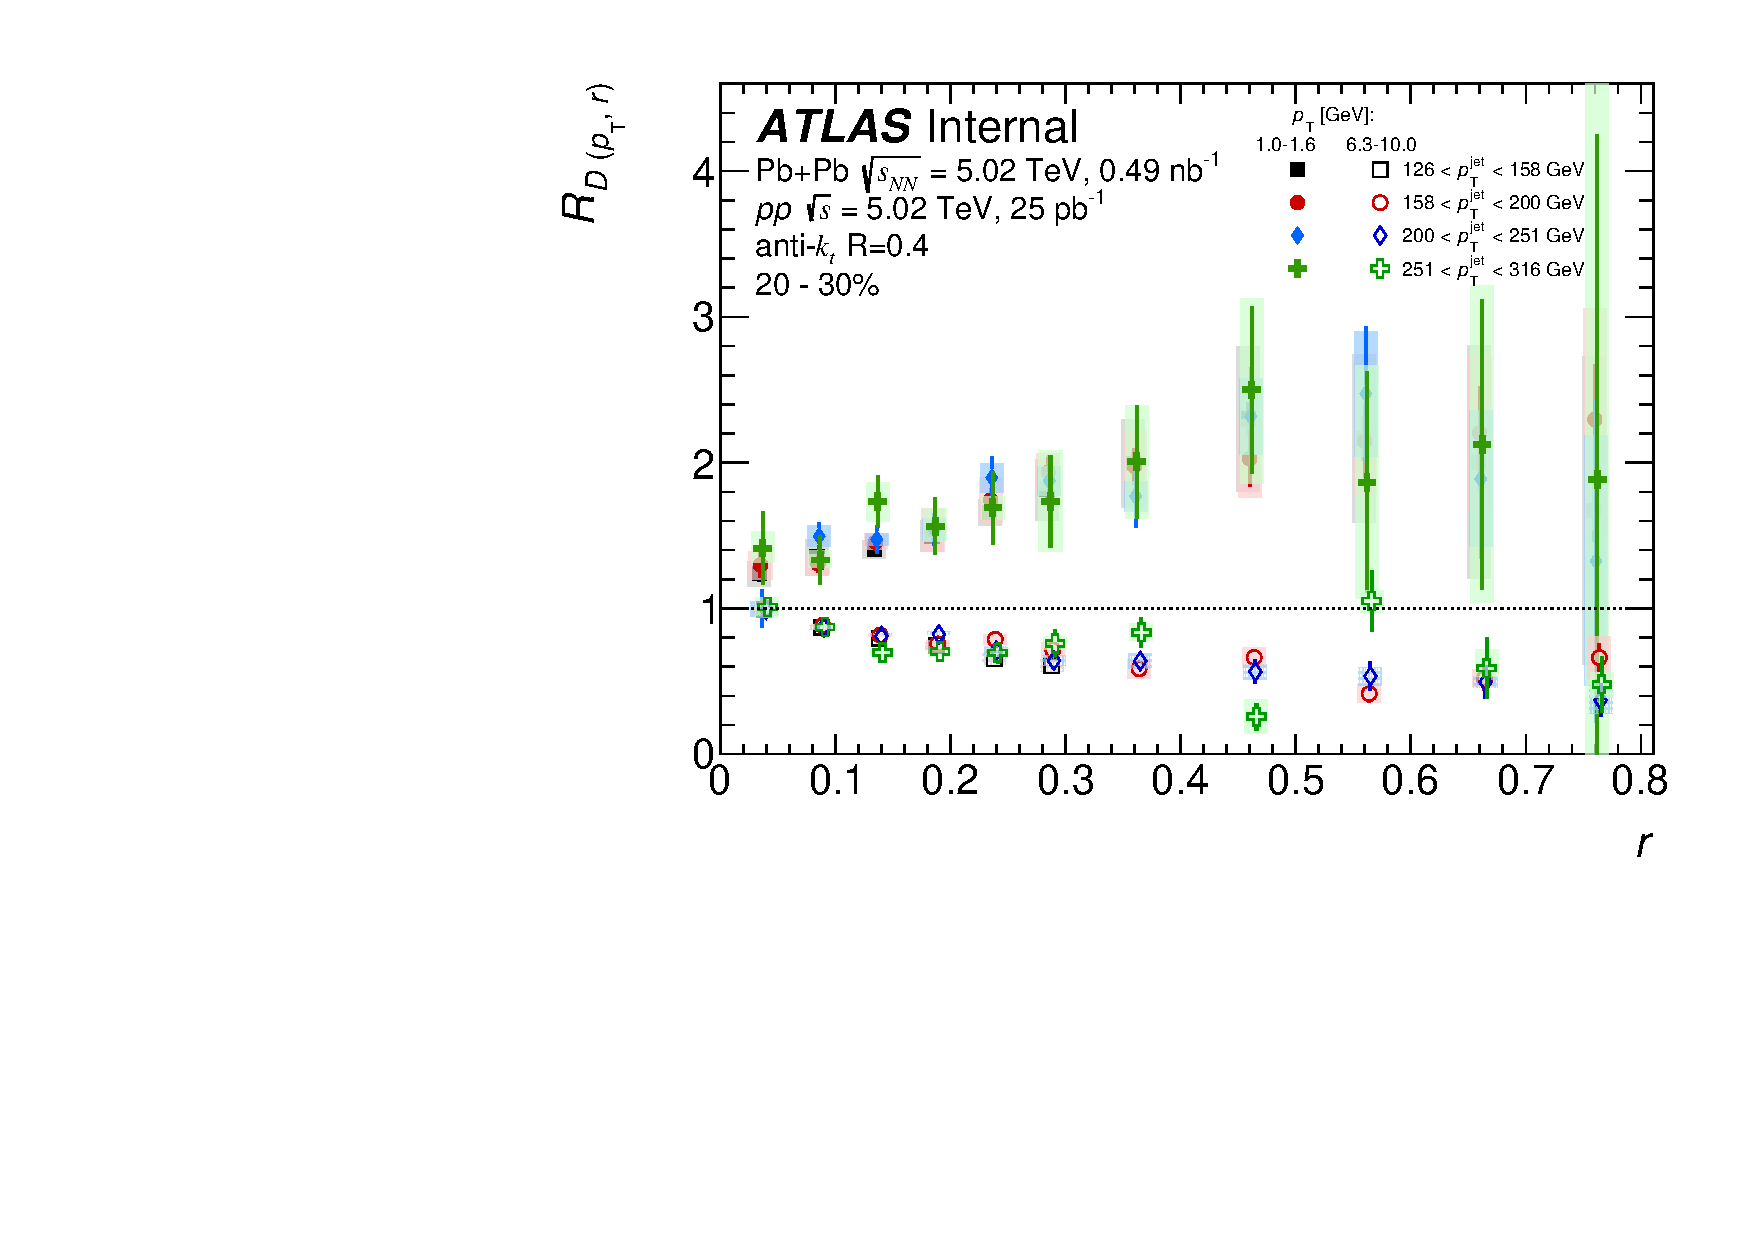
\includegraphics[width=0.45\textwidth]{figures_results/RDpT_final_ratio_dR_CONF_data_trk2_6_cent2} &
	 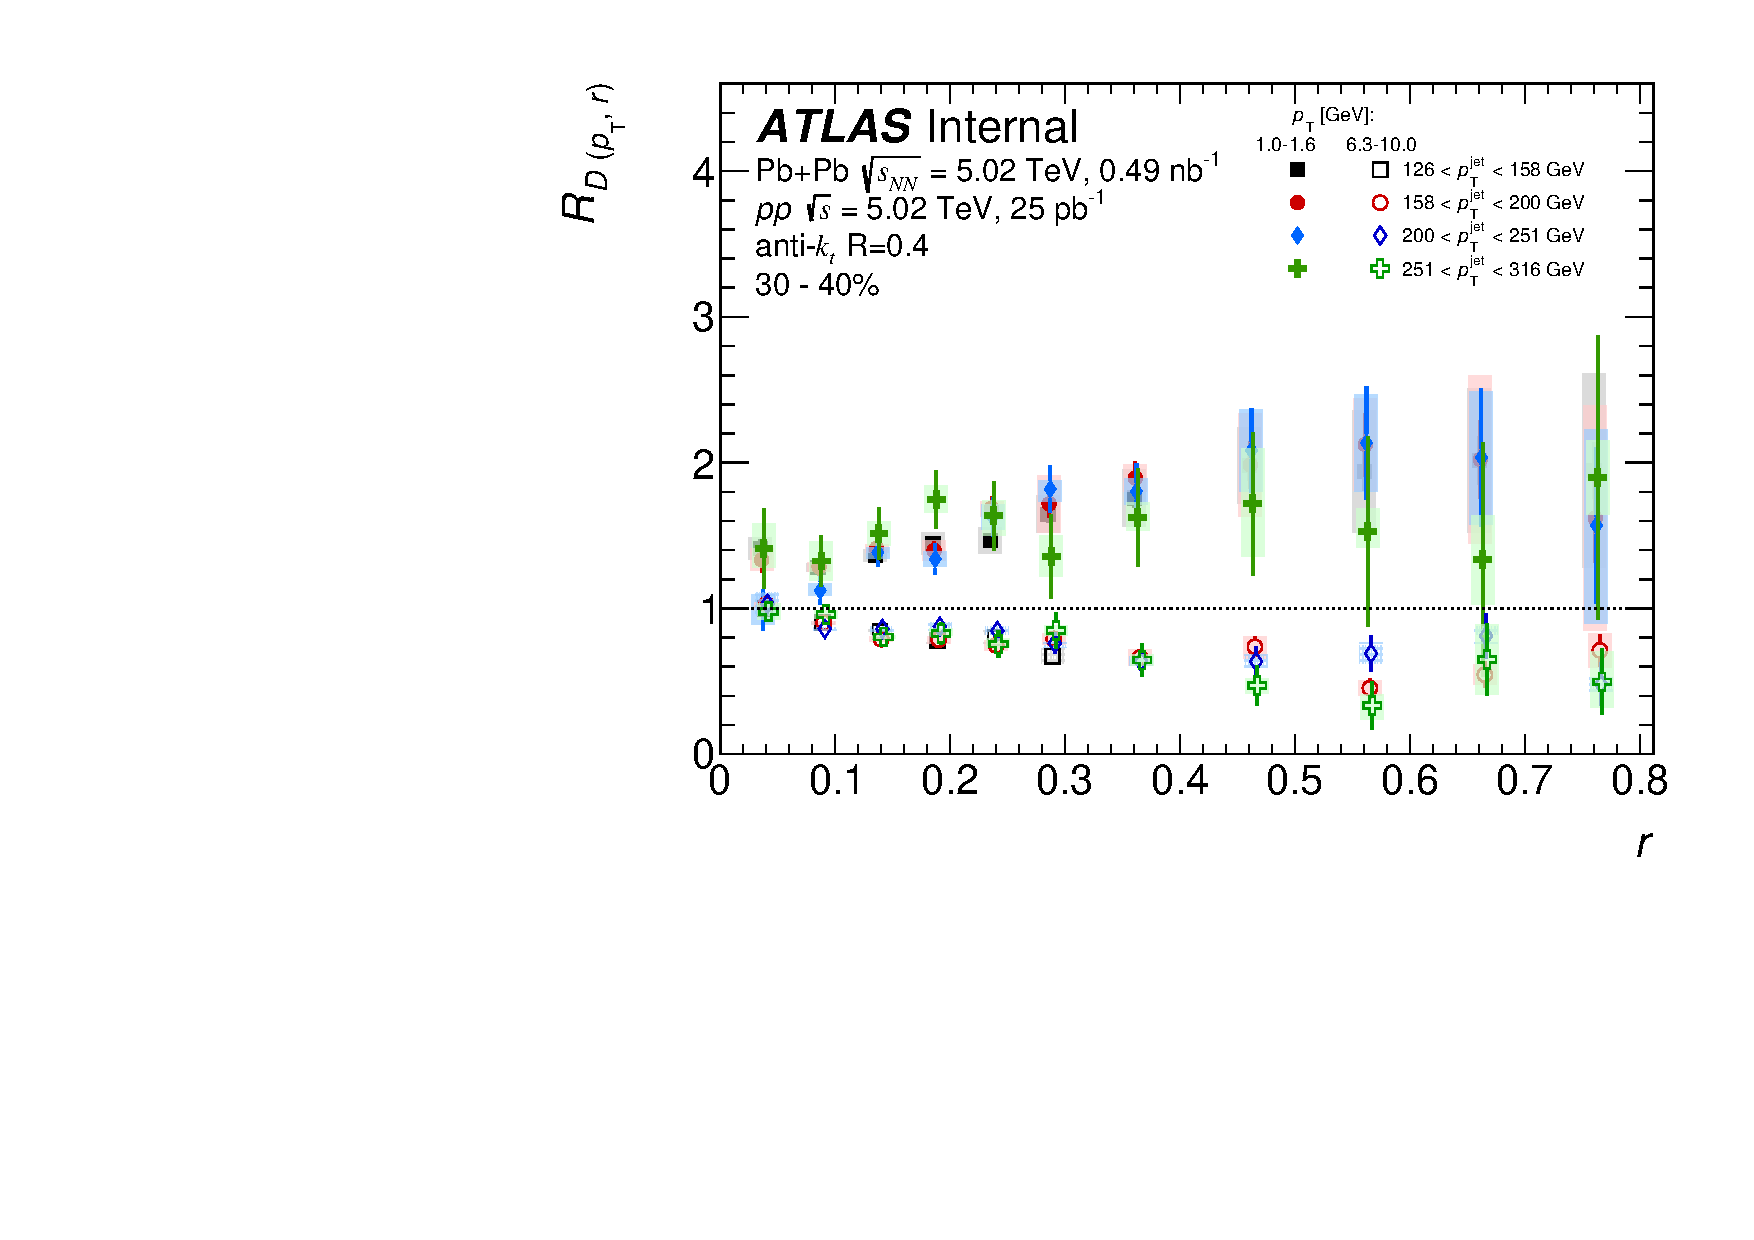
\includegraphics[width=0.45\textwidth]{figures_results/RDpT_final_ratio_dR_CONF_data_trk2_6_cent3} \\
	 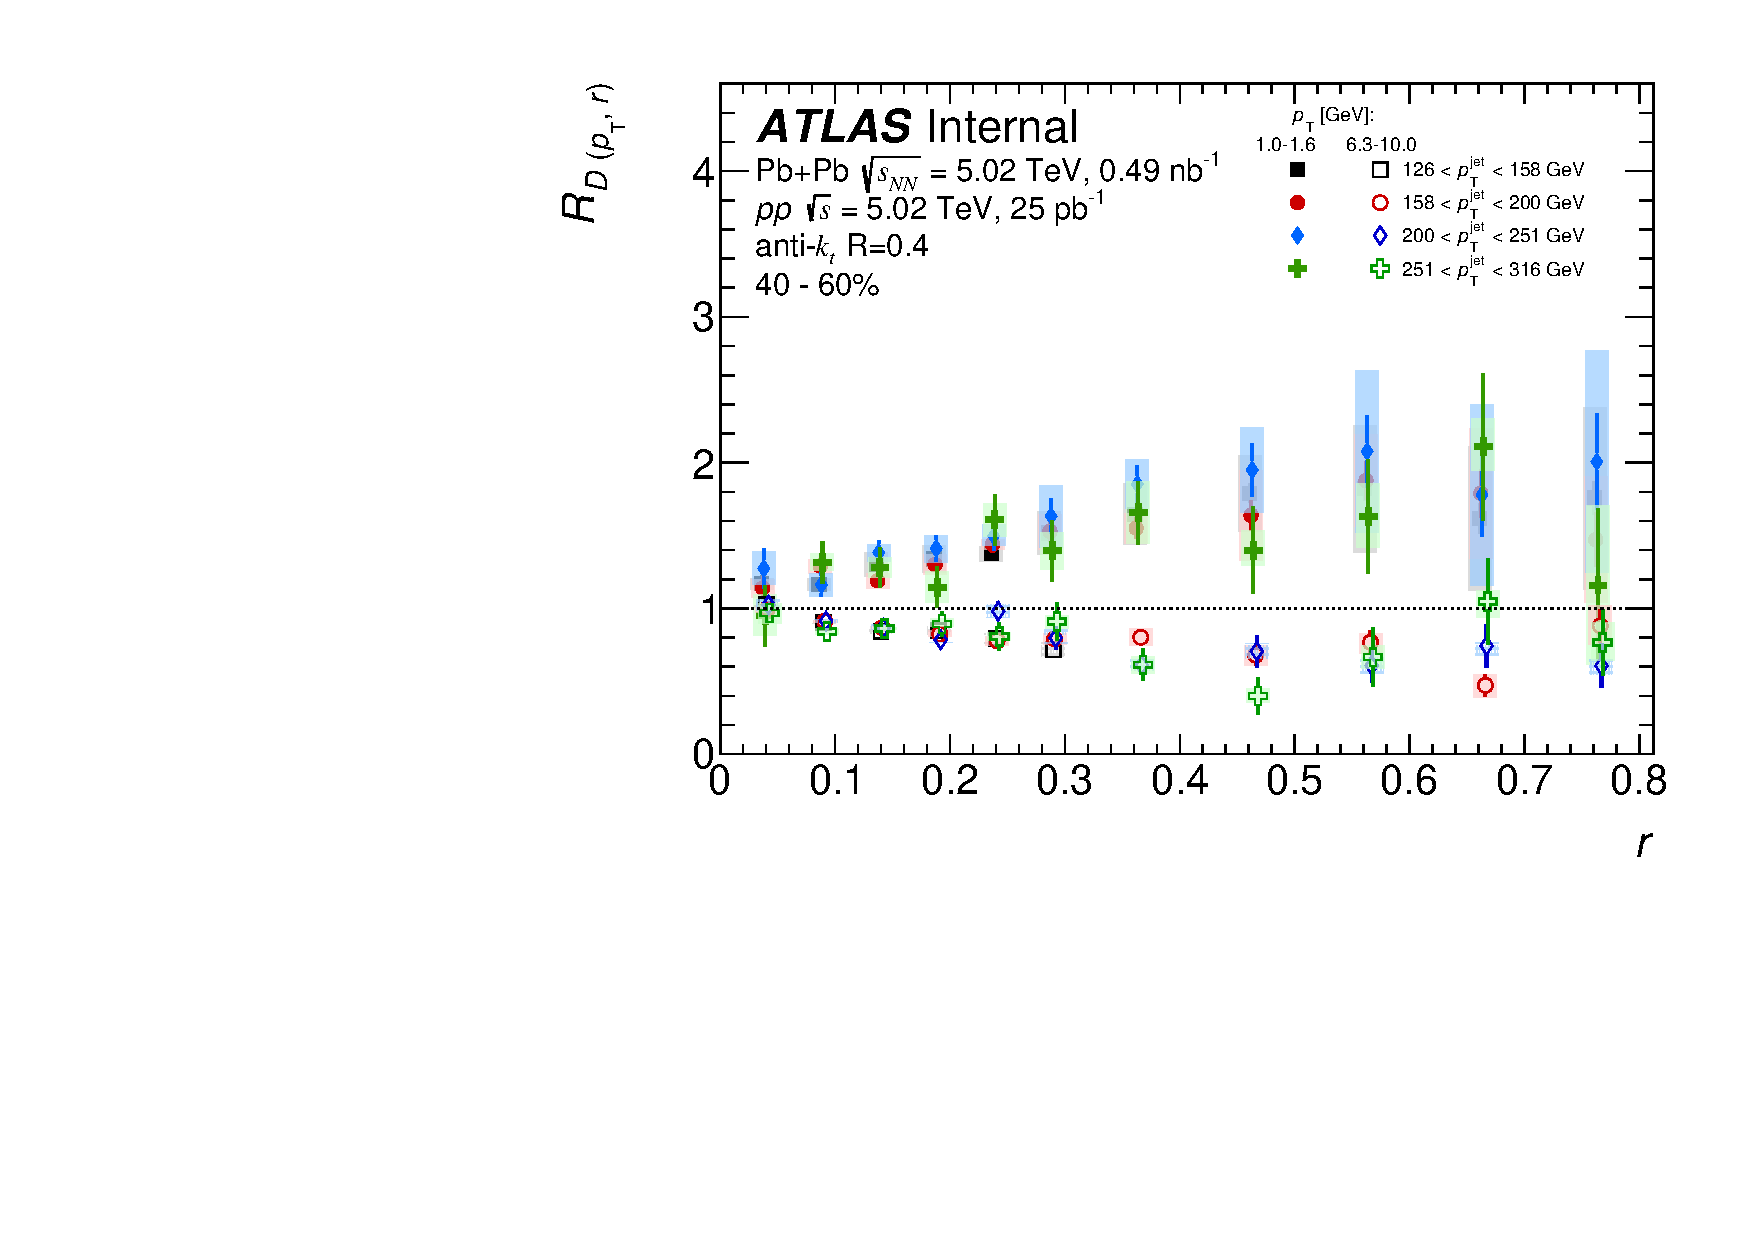
\includegraphics[width=0.45\textwidth]{figures_results/RDpT_final_ratio_dR_CONF_data_trk2_6_cent4} &
	 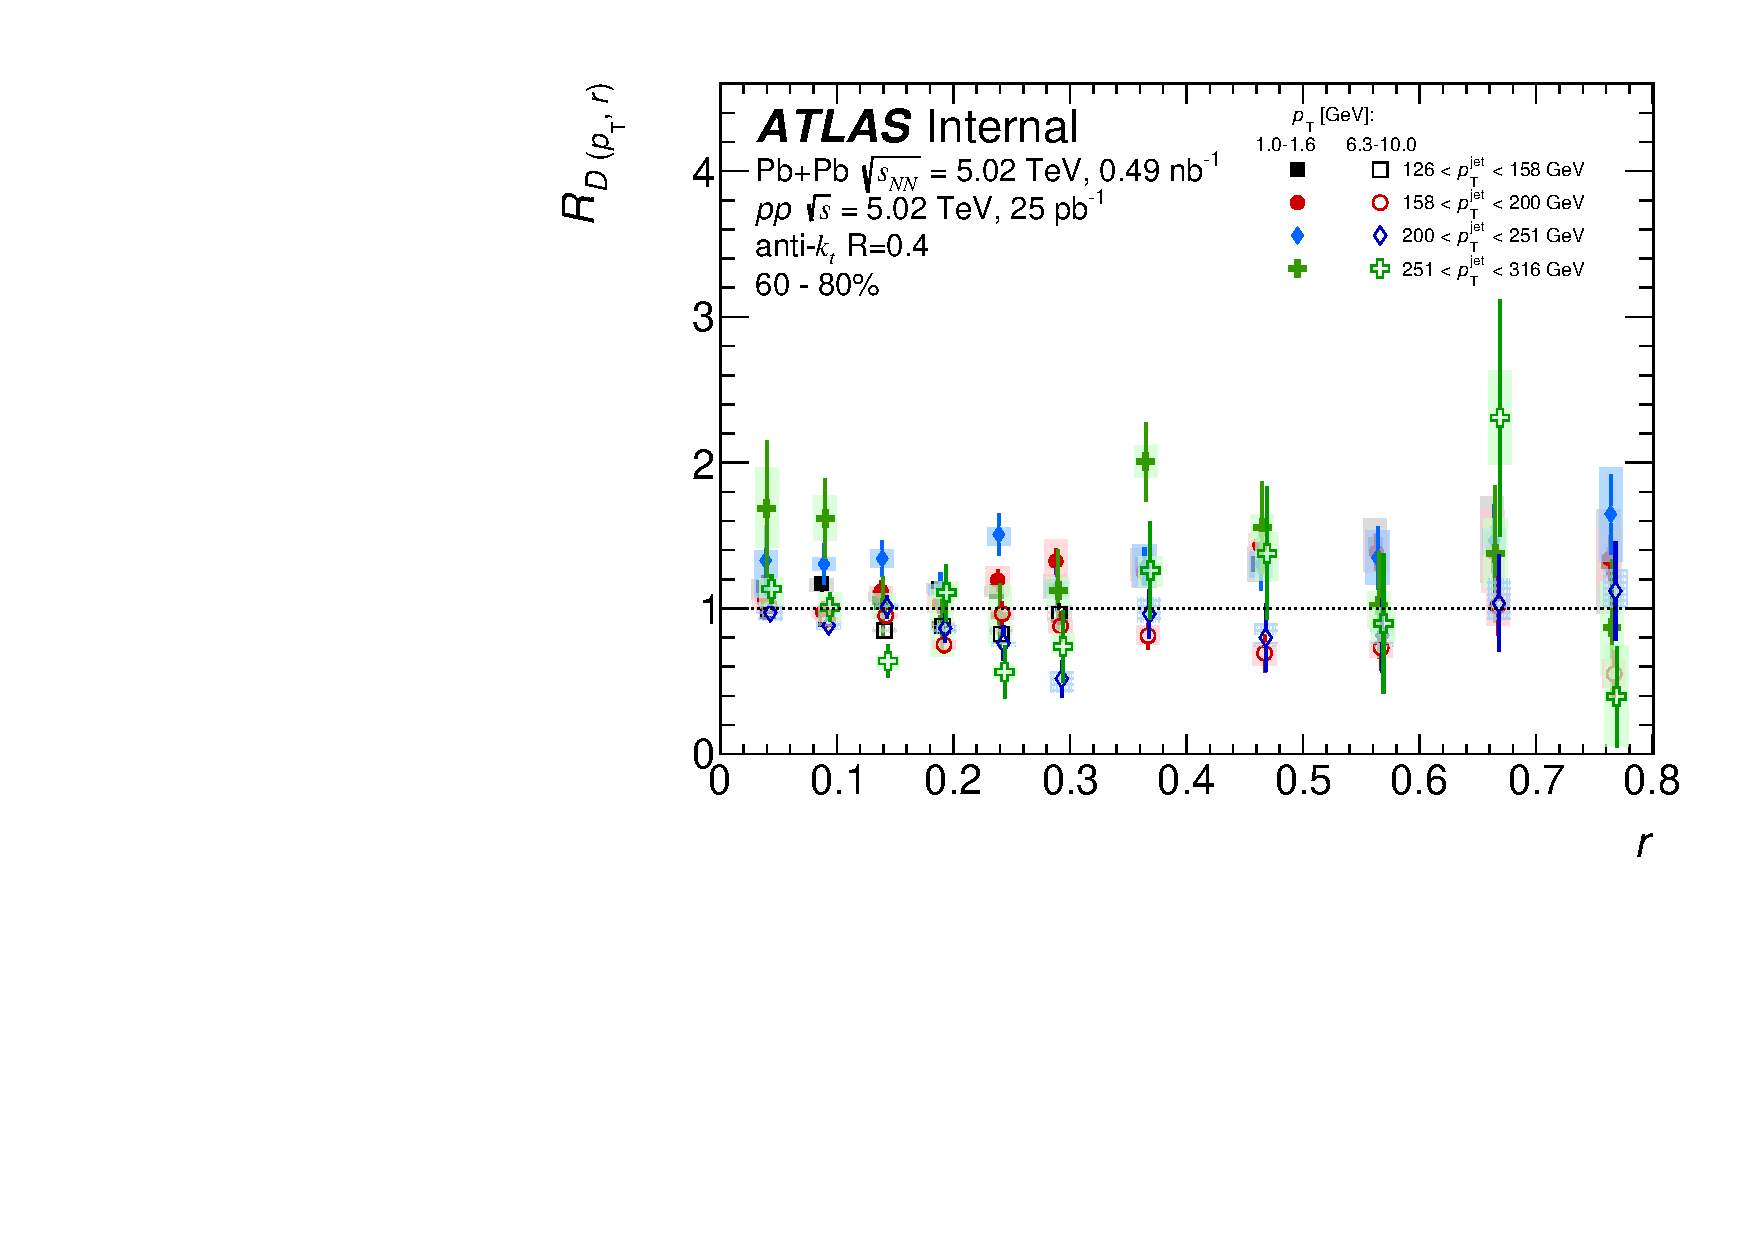
\includegraphics[width=0.45\textwidth]{figures_results/RDpT_final_ratio_dR_CONF_data_trk2_6_cent5} \\
\end{tabular} }
   \caption{\RDptr\ as a function of \rvar\ for different centrality bins for charged particles with \mbox{$1.0 < \pt < 1.6$ \GeV}
(filled points) and $6.3 < \pt < 10.0 $ \GeV\ (open points) for four \ptjet\ selections: 126--158~\GeV, 158--200~\GeV,
200--251~\GeV, and 251--316~\GeV.}
      \label{fig:ptjetdep}
\end{figure}



It can be seen that in most central collisions, yields of low \pt\ charged particles ($\pttrk \lesssim 4$ GeV) is enhanced in \PbPb\ collisions compared to \pp\ collisions for $r \lesssim 0.8$. This excess is monotonically increasing from $r=0$, reaching the maximum around $r\approx0.4$ and then decreasing. Yields of higher \pt\ particles with $\pttrk \gtrapprox 4$ GeV show are suppressed in \PbPb\ collisions compared to the \pp\ reference across the entire $r$ range except for the core of the jet. This can be seen more clearly in Fig.\ref{fig:RDpT_wrt_trk}, where the jet core shows no suppression across the entire track \pt\ range under investigation. Any deviations from unity in the \RDptr distributions come only from tracks not in the jet core. This is in the agreement with the observation in the measurement of the inclusive jet fragmentation functions where the yields of the high-$\pT$ fragments are observed to be enhanced in \PbPb\ collisions compared to the \pp\ reference~\cite{ATLAS502FFConf}. This enhancement of fragment yields with high $\pt$ was recently discussed in terms of the expected stronger quenching of  gluon jets than quark jets~\cite{Spousta:2015fca} and within a hybrid strong/weak coupling model of jet quenching~\cite{Hulcher:2017cpt}.  The size of the modification to the charged particles yields gradually decreasing with the  decreasing collisions centrality. Furthermore, the magnitude of the excess of low transverse momentum particles increases with increasing jet transverse momentum. The enhancement of fragment yields at low \pT\ is consistent with models of the jet quenching where the energy lost by fast partons is transferred predominantly to soft particles outside the jet cone and it might result from the response of the medium to the partonic shower. This is further suggested by the observation of dependence of the magnitude of excess on the jet \pt.

\begin{figure}
\centering{
\begin{tabular}{cc}
	 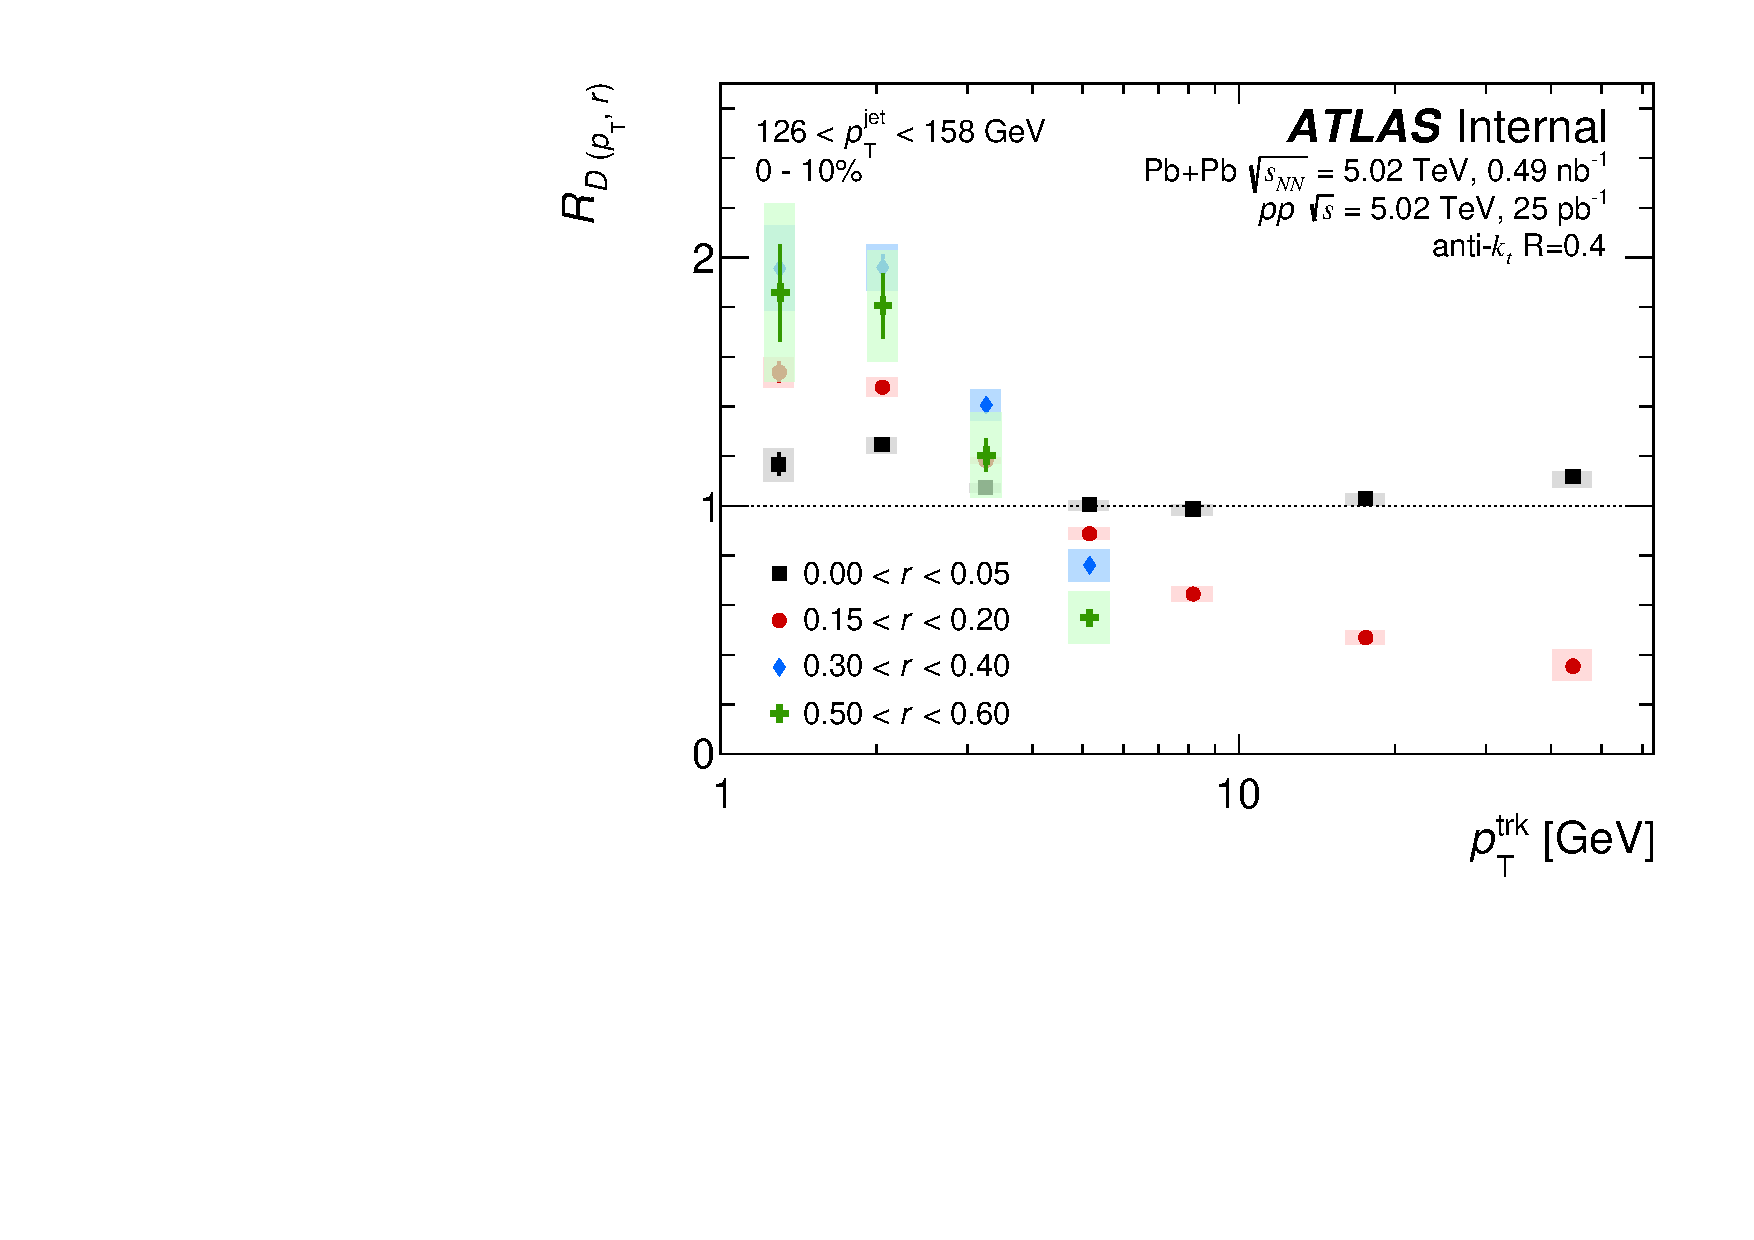
\includegraphics[width=0.45\textwidth]{figures_results/RDpT_final_ratio_dR_CONF_data_trkpT_jet7_cent0} &
	 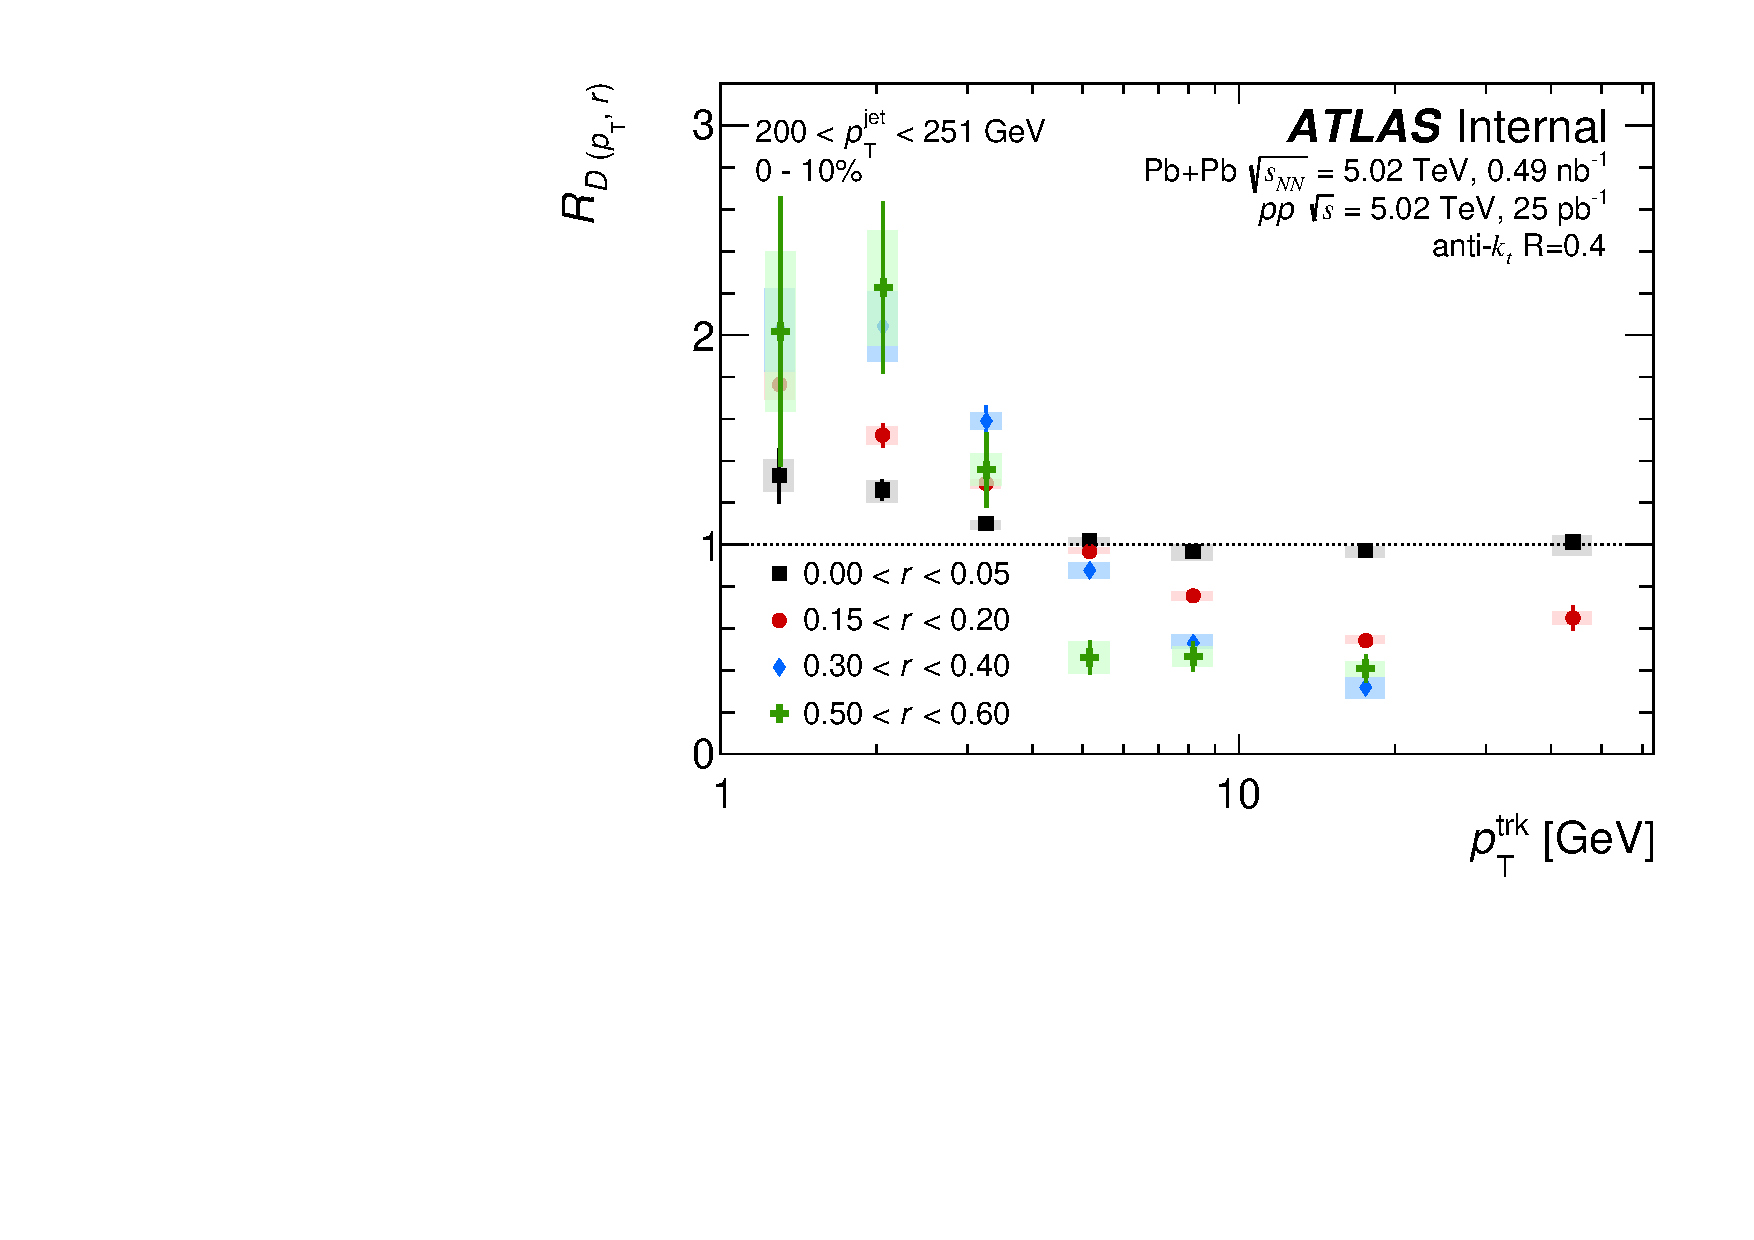
\includegraphics[width=0.45\textwidth]{figures_results/RDpT_final_ratio_dR_CONF_data_trkpT_jet9_cent0} \\
	 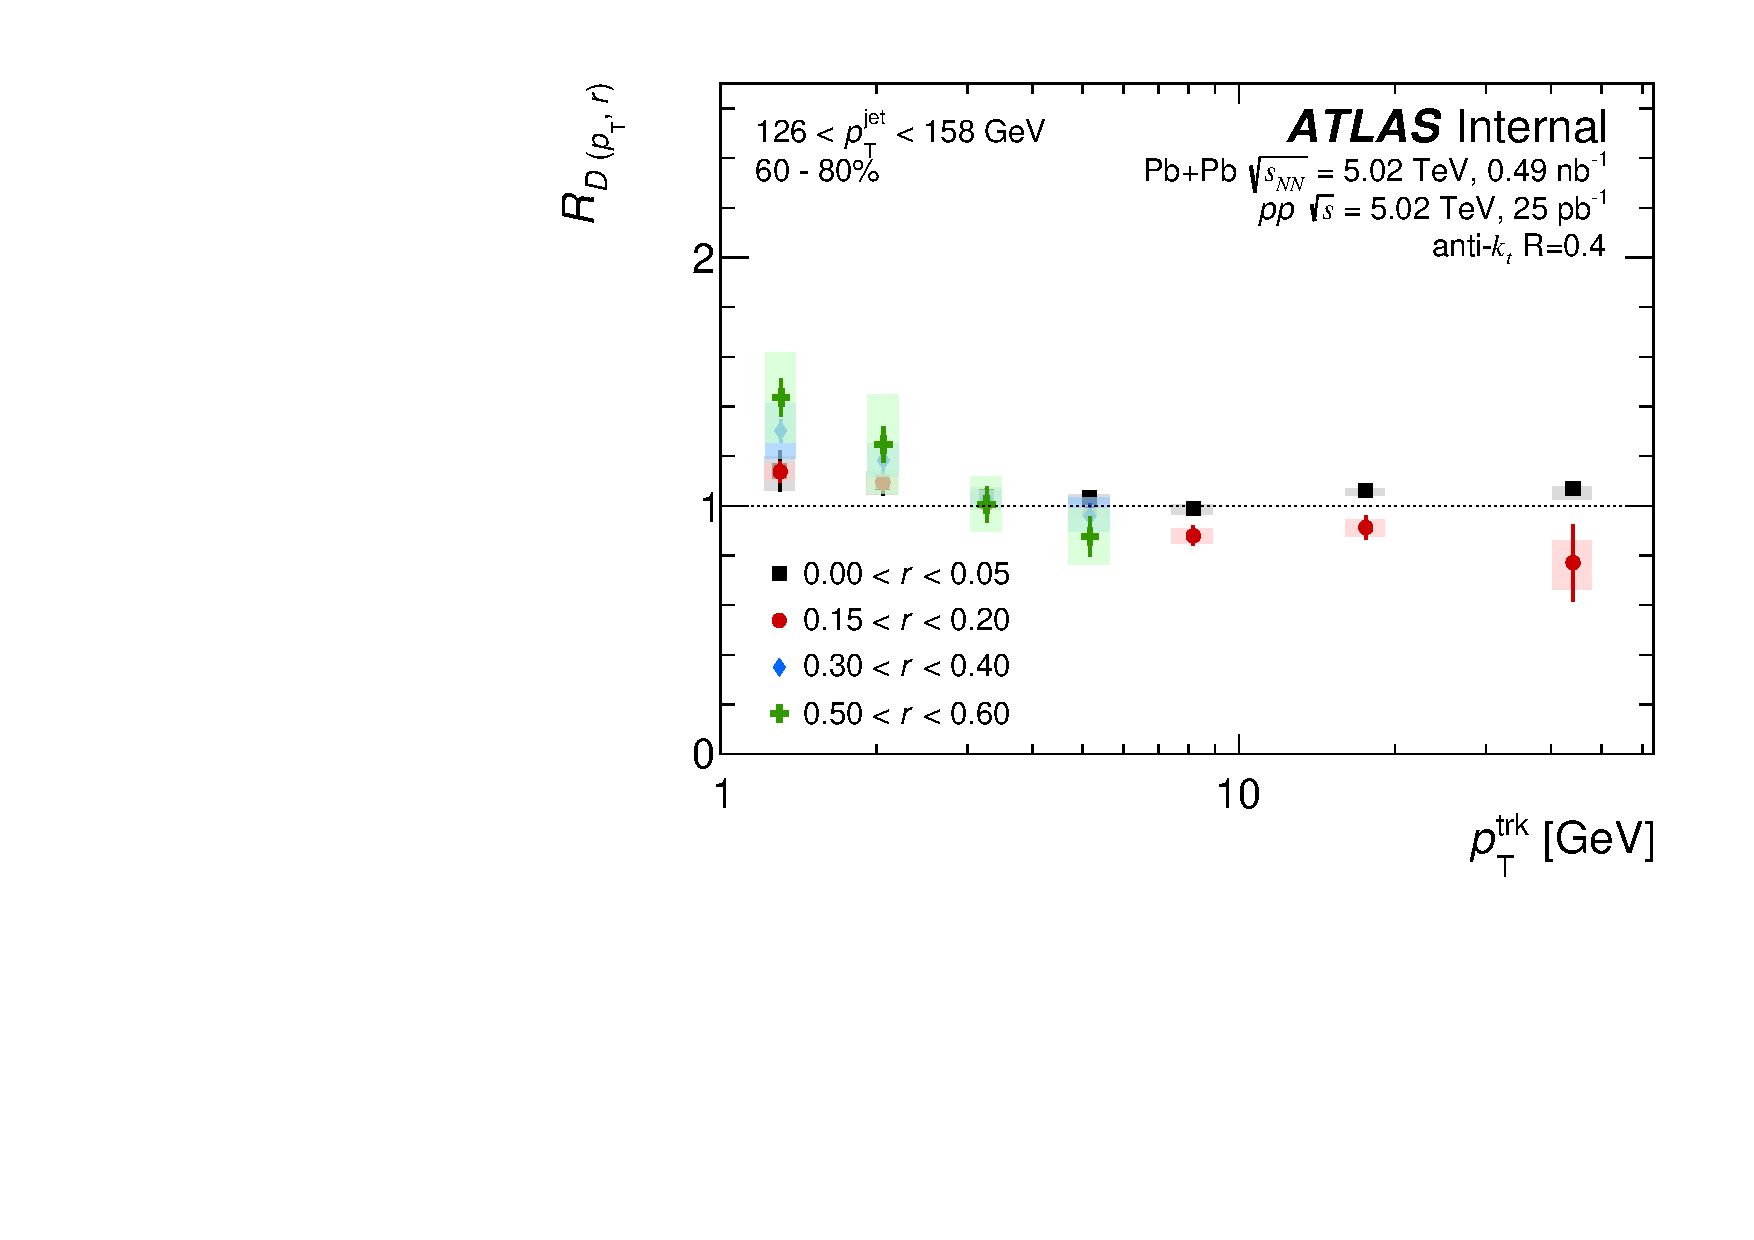
\includegraphics[width=0.45\textwidth]{figures_results/RDpT_final_ratio_dR_CONF_data_trkpT_jet7_cent5} &
	 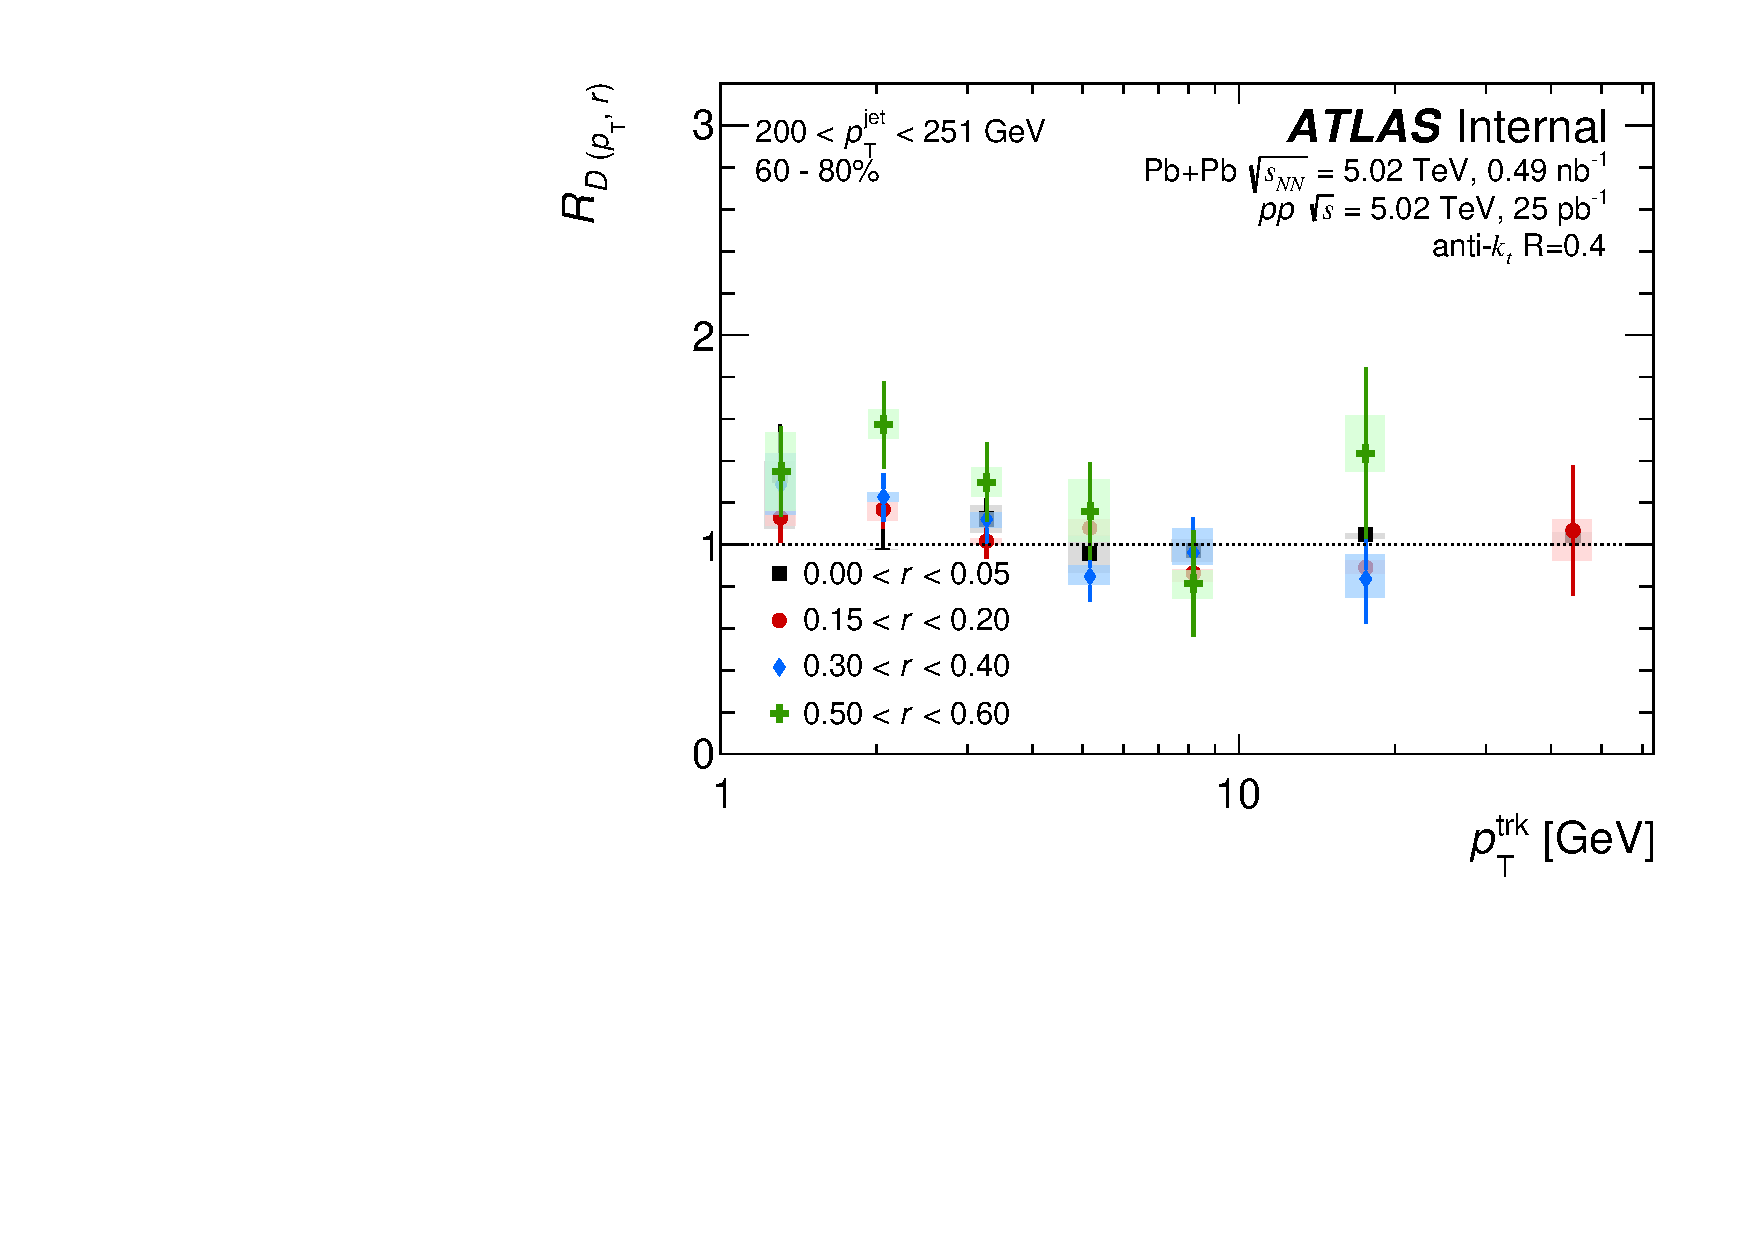
\includegraphics[width=0.45\textwidth]{figures_results/RDpT_final_ratio_dR_CONF_data_trkpT_jet9_cent5} \\
\end{tabular} }
   \caption{\RDptr\ as a function of \pt\ in central (top) and peripheral (bottom) collisions for two different \ptjet\ selections: 126--158~\GeV\ (left) and 200--251~\GeV\ (right). The different colors indicate different distances from the jet axis}
      \label{fig:RDpT_wrt_trk}
\end{figure}


The difference between the \Dptr\ distributions in \pp\ and \pbpb, $\Delta\Dptr$, for 126--158~\GeV\  and 200--251 \GeV\ jets in the most central collisions can be can be seen in Fig.\ref{fig:DeltaDptr}. The uncertainties do not cancel between the two collision systems.
% While the relative uncertainties on the \Dptr\ distributions are largest at large \rvar\ (as seen in Fig.\ref{fig:dptr_sys_uncert_A1}-\ref{fig:dptr_sys_uncert_A3}) the absolute uncertainties are larger in the jet core, where the signal is larger. 
The $\Delta\Dptr$ distributions indicate an excess (depletion) in the number of particles in the \pbpb\ system compared to the \pp\ system for low (high) \pt\ particles. This excess ranges from 0.5 to 4 particles for 1 \GeV\ tracks while the depletion ranges from $\sim$0 to 0.5 particles for 10 \GeV\ tracks. An increase in the extra number of particles with increasing \ptjet\ for low \pt\ tracks is also seen. The relative uncertainties on the $\Delta\Dptr$ distributions can be seen in Fig.\ref{fig:deltadptr_sys_uncert_A1}-\ref{fig:deltadptr_sys_uncert_A3}


\begin{figure}
\centering{
\begin{tabular}{cc}
	 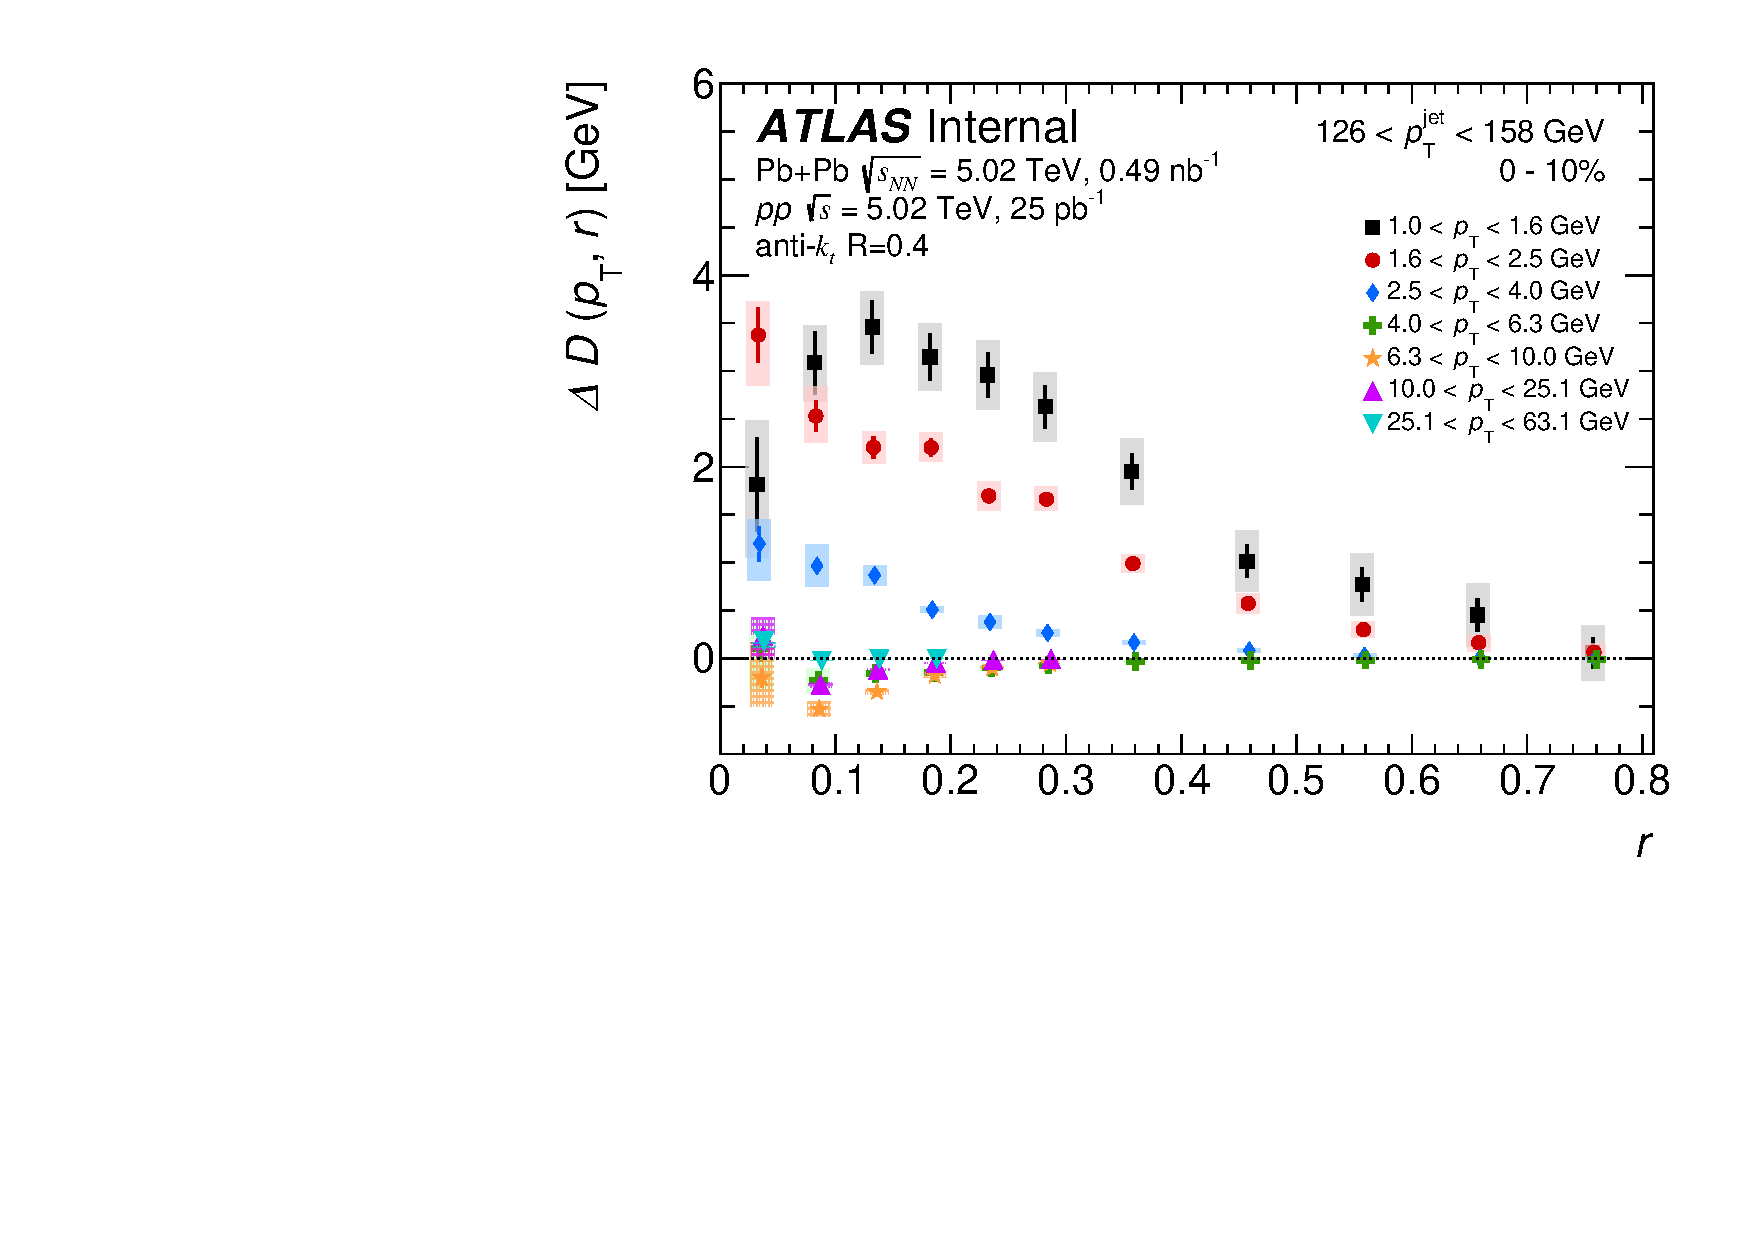
\includegraphics[width=0.45\textwidth]{figures_results/DeltaDpT_final_ratio_dR_CONF_data_jet7_cent0} &
	 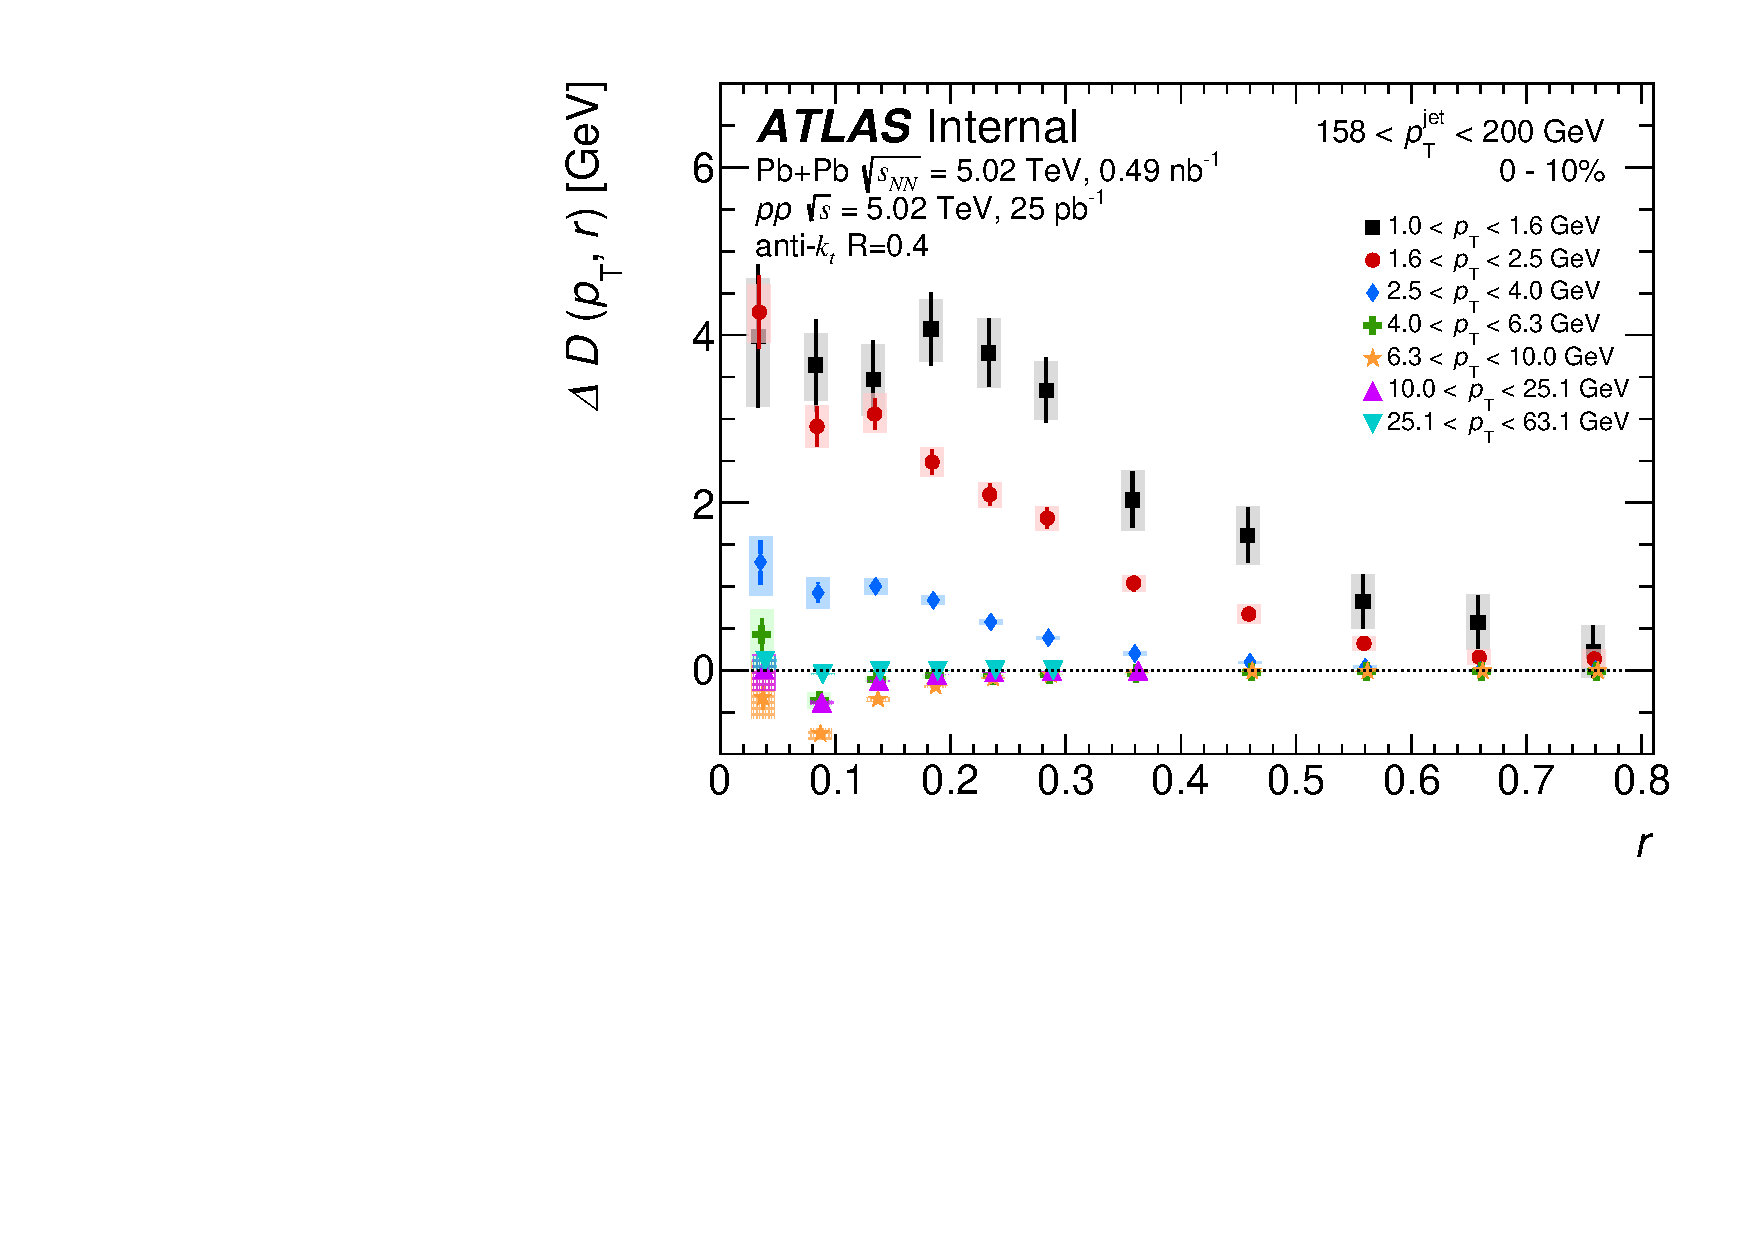
\includegraphics[width=0.45\textwidth]{figures_results/DeltaDpT_final_ratio_dR_CONF_data_jet8_cent0} \\
	 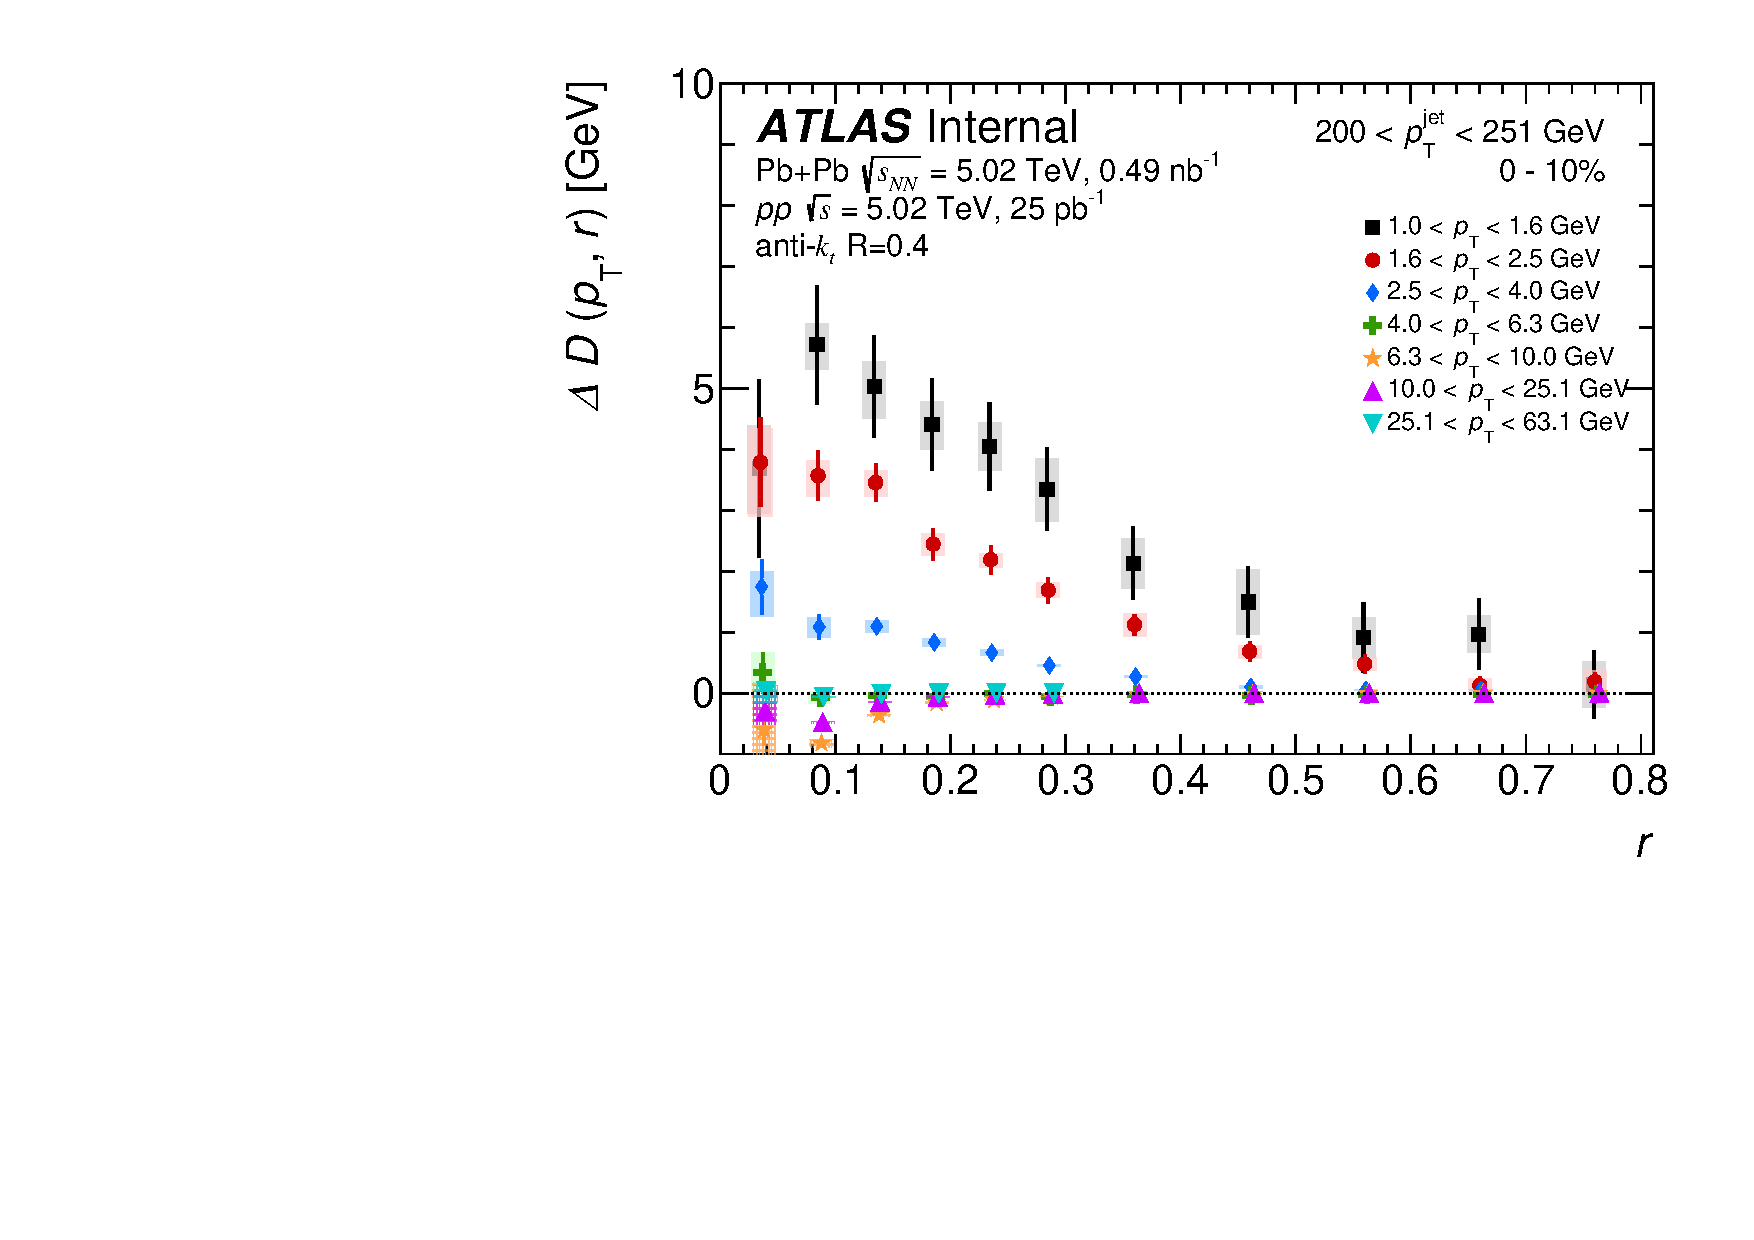
\includegraphics[width=0.45\textwidth]{figures_results/DeltaDpT_final_ratio_dR_CONF_data_jet9_cent0} &
	 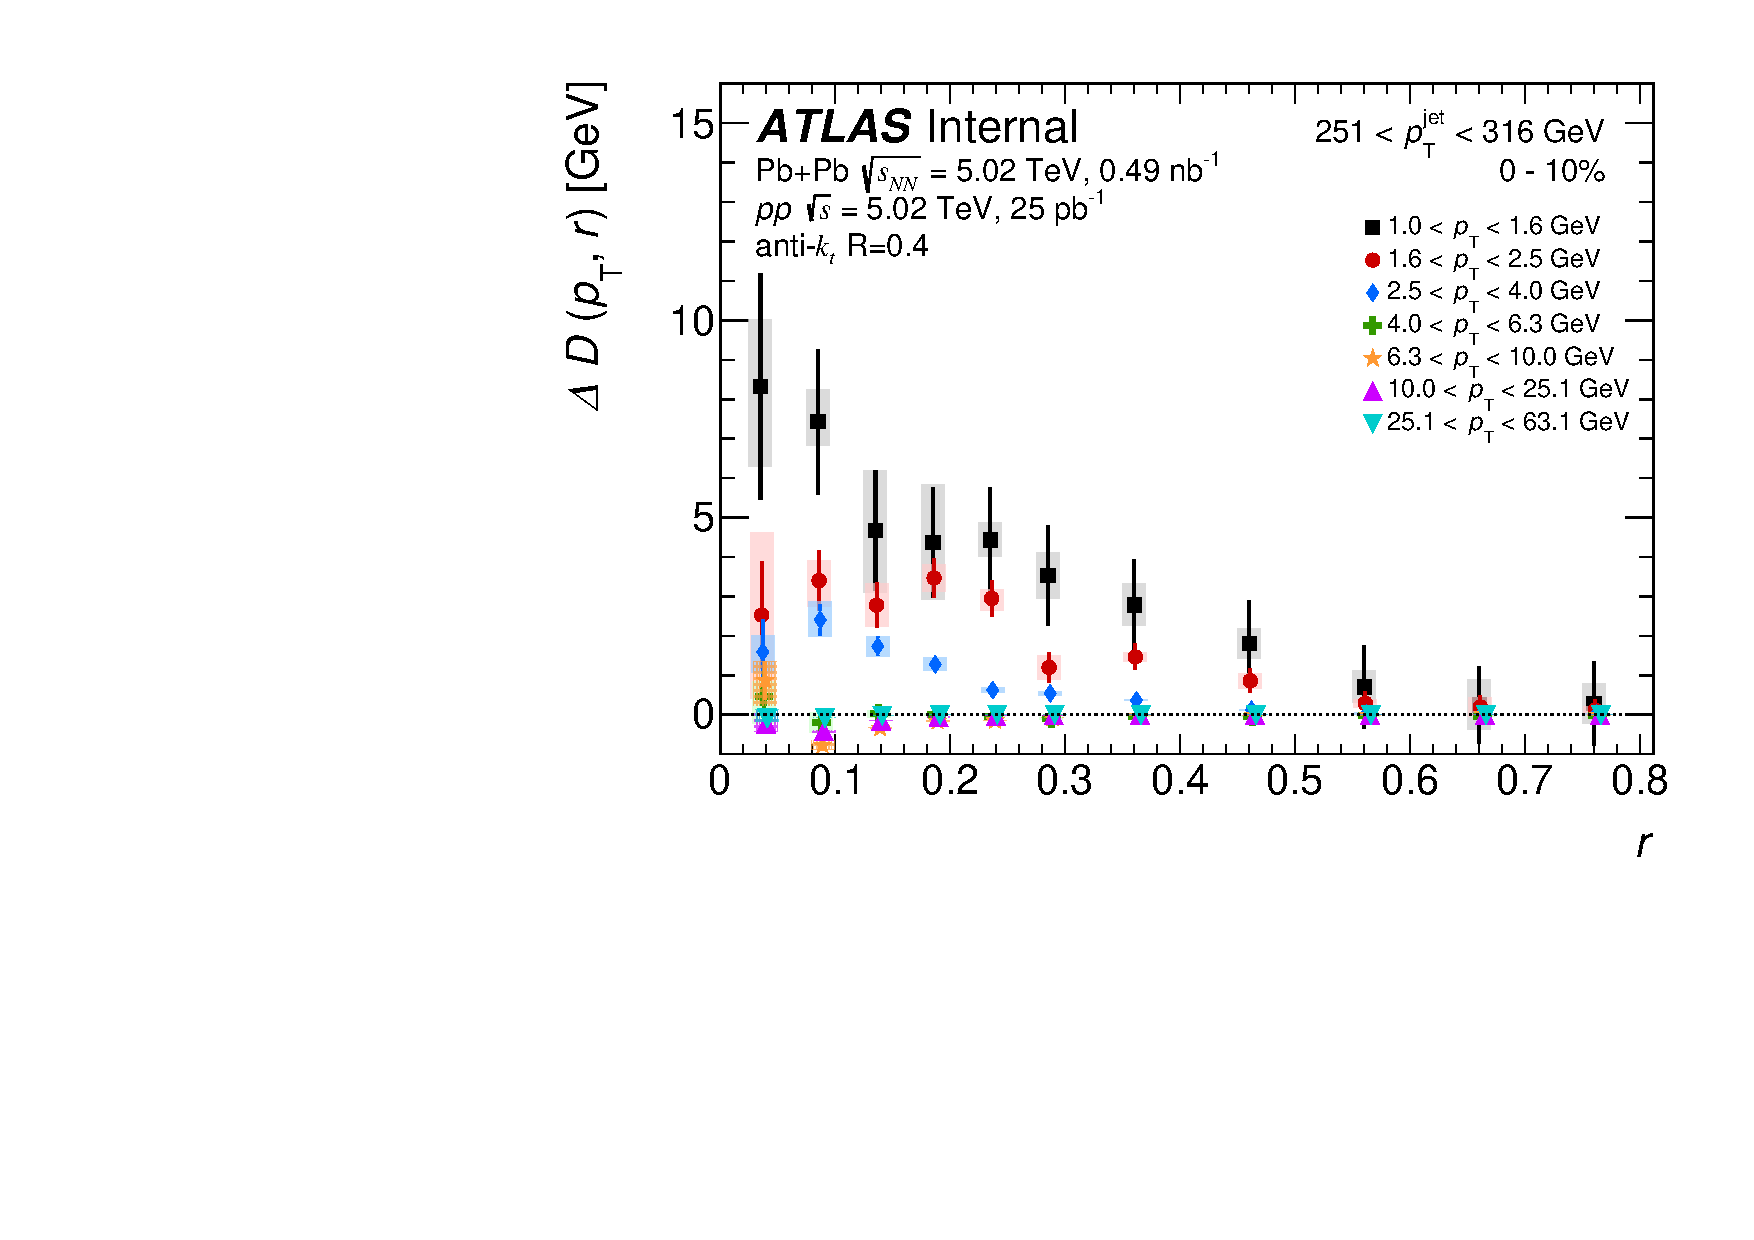
\includegraphics[width=0.45\textwidth]{figures_results/DeltaDpT_final_ratio_dR_CONF_data_jet10_cent0} \\
\end{tabular} }
   \caption{$\Delta \RDptr$ as a function of \rvar\ in central collisions for all \pt\ ranges in four \ptjet\ selections: 126--158~\GeV, 158--200~\GeV, 200--251~\GeV, and 251--316~\GeV. }
      \label{fig:DeltaDptr}
\end{figure}





%%%%%%%%%%%%%%%%%%%%%%%
